% ELABORAZIONE ITERAZIONE 3 - UC4_SendPrivateMessage
\section{Elaborazione - Iterazione 3}
\begin{frame} {Descrizione Elaborazione: Iterazione 3}
  \begin{scriptsize}
    In questa terza iterazione è stato sviluppato il caso d'uso relativo all'invio del messaggio privato. Rispetto al class diagram precedentemente è stata aggiunta 
    la classe PrivateMessage nel package Common. Tale classe, come la classe Notify, Command e PublicMessage, è una sottoclasse di Message avente come attributo 
    aggiuntivo il nickname del destinatario a cui è indirizzato il messaggio privato.
    \newline
    Per la gestione dei messaggi privati sono state modificate le interfacce IUser in cui è stato inserito un metodo per la ricezione dei messaggi privati, e   
    IMessagingService nella quale invece è stato inserito un metodo per l'invio dei messaggi privati. Anche l'interfaccia IUserInteraction verrà modificata per 
    permettere la visualizzazione nell'interfaccia utente del messaggio privato.
  \end{scriptsize}
\end{frame}

\subsection {Iterazione 3: Requisiti - UC4\_SendPrivateMessage}
\begin{frame} {Iterazione 3: Requisiti - UC4\_SendPrivateMessage}
  \begin{table}[!htbp]
    \caption {Caso d'uso UC4\_SendPrivateMessage}
     \label{table_UC4_SPM}
      \resizebox{\linewidth}{!}{%
       \begin{tabular}{|l|p{10cm}|}\hline
        Nome caso d'uso &  UC3\_SendRoomMessage\\\hline
        Portata & Applicazione Smart Intelligent University Communications \\\hline
        Livello & Obiettivo Utente \\\hline
        Attore primario & SnucUser  \\\hline
        Parti interessate e interessi & SnucUser: vuole che i messaggi siano inviati all’utente selezionato presente nella stanza virtuale \\\hline
        Pre-condizioni &  L'utente è registrato nella stanza in cui desidera inviare un messaggio ad un altro utente presente \\\hline
        Post-condizioni (garanzia di successo) & L'utente selezionato riceve il messaggio inviato \\\hline
         Scenario principale di successo &  
         \begin{enumerate} 
          \item L’utente seleziona il destinatario del messaggio privato.
          \item L’utente inserisce da tastiera il messaggio da inviare.
	  \item Il messaggio viene inoltrato al destinatario selezionato.
         \end{enumerate} \\\hline
      \end{tabular}}
   \end{table}
\end{frame}

\begin{frame} {Iterazione 3: Requisiti - UC4\_SendPrivateMessage}
  \begin{table}[!htbp]
      \resizebox{\linewidth}{!}{%
       \begin{tabular}{|l|p{10cm}|}\hline
         Requisiti speciali (Requisiti Non Funzionali) &  Comunicazione asincrona in cui lo scambio di informazioni avviene in tempo reale, senza sensibili pause tra 
                                                        invio e ricezione del messaggio\\\hline
         Elenco delle varianti tecnologiche &  
          \begin{itemize}  
           \item \`E possibile inviare messaggi confidenziali, autenticati e integri al server del servizio di messaggistica.
           \item L’applicazione dovrebbe essere flessibile al funzionamento di diversi protocolli di comunicazione (es. TCP, UDP) e con diversi strati middleware 
                 (es. Socket, RMI)
          \end{itemize} \\\hline
         Frequenza di ripetizione & Potrebbe essere quasi ininterrotta \\\hline
         Varie e/o Problemi Aperti &  // \\\hline
      \end{tabular}}
   \end{table}
\end{frame}

\subsection {Iterazione 3: Analisi - UC4\_SendPrivateMessage}
\begin{frame} [allowframebreaks] {Descrizione Iterazione 3: Analisi - UC4\_SendPrivateMessage}
  In questa iterazione, del caso d’uso UC4 è di interesse lo scenario principale di successo.  Da esso è possibile identificare le seguenti classi concettuali: 
  \begin{itemize}
   \item \textbf{User}: rappresenta il generico utente, caratterizzato da un ``nickname'', connesso al servizio di messaggistica. Può richiedere la lista delle 
         stanze, ricevere notifiche dal sistema centrale. Interagisce con il MessagingSevice richiedendo la registrazione e l’ingresso in una specifica stanza. 
         Può inviare messaggi pubblici e \textit{privati}.
   \item \textbf{MessagingService}: rappresenta ed incapsula il servizio di messaggistica nel suo complesso. Mantiene una lista di utenti connessi a tale sistema. 
          Mantiene una lista di stanze e riceve tramite comandi richieste di ingresso da parte degli utenti. Svolge il ruolo di smistatore di messaggi inviati dagli 
          User.
   \item \textbf{Message}: individua un generico messaggio scambiato tra utenti della chat o tra servizio di messaggistica e utente. È costituito da un 
         ``content'' (contenuto del messaggio) , da una ``date'' (rappresenta la data) e dal ``sender'' (mittente).
   \item \textbf{Notify}: è una specializzazione del tipo Message ed è caratterizzata da un typeNotify che serve a distinguere il tipo di notifica (ad es. 
          CONNECTIO\_ACCEPT nel caso in cui la connessione è stata stabilita correttamente, BAD\_COMMAND nel caso in cui il comando inviato dall'User non 
          sia riconosciuto dal Server).
   \item \textbf{PublicNotify}: è una specializzazione di Notify e questo tipo di notifica viene ricevuta da tutti gli utenti registrati alla relativa 
          stanza. Un esempio di PublicNotify è la notifica caratterizzata dal seguente typeNotify: UPDATE\_LIST\_USERS, grazie alla quale viene 
          aggiornata la lista degli utenti registrati nella relativa stanza.
   \item  \textbf{Commad}: è una specializzazione di Message e rappresenta il comando che viene inviato dall'User e ricevuto ed interpretato dal            
          MessagingService (es. /join '\#Medical' richiesta da parte dell'utente a registrarsi alla stanza Medical).        
   \item \textbf{Room}: è caratterizzata da un nome. Ciascuna istanza individua una specifica stanza nella chat.
   \item \textbf{Register}: mantiene un riferimento all’insieme di partecipanti che in un certo istante sono presenti nella stanza.
   \item \textbf{PublicMessage}: è una specializzazione di Message ed individua un messaggio pubblico scambiato tra utenti della chat registrati nella 
         stessa stanza. 
   \item \textit{\textbf{PrivateMessage}: una specializzazione di Message ed individua un messaggio privato scambiato tra due utenti della chat registrati nella  
         stessa stanza}. 
  \end{itemize}
\end{frame}

\begin{frame} {Iterazione 3: Analisi - UC4\_SendPrivateMessage}
   \begin{figure}
     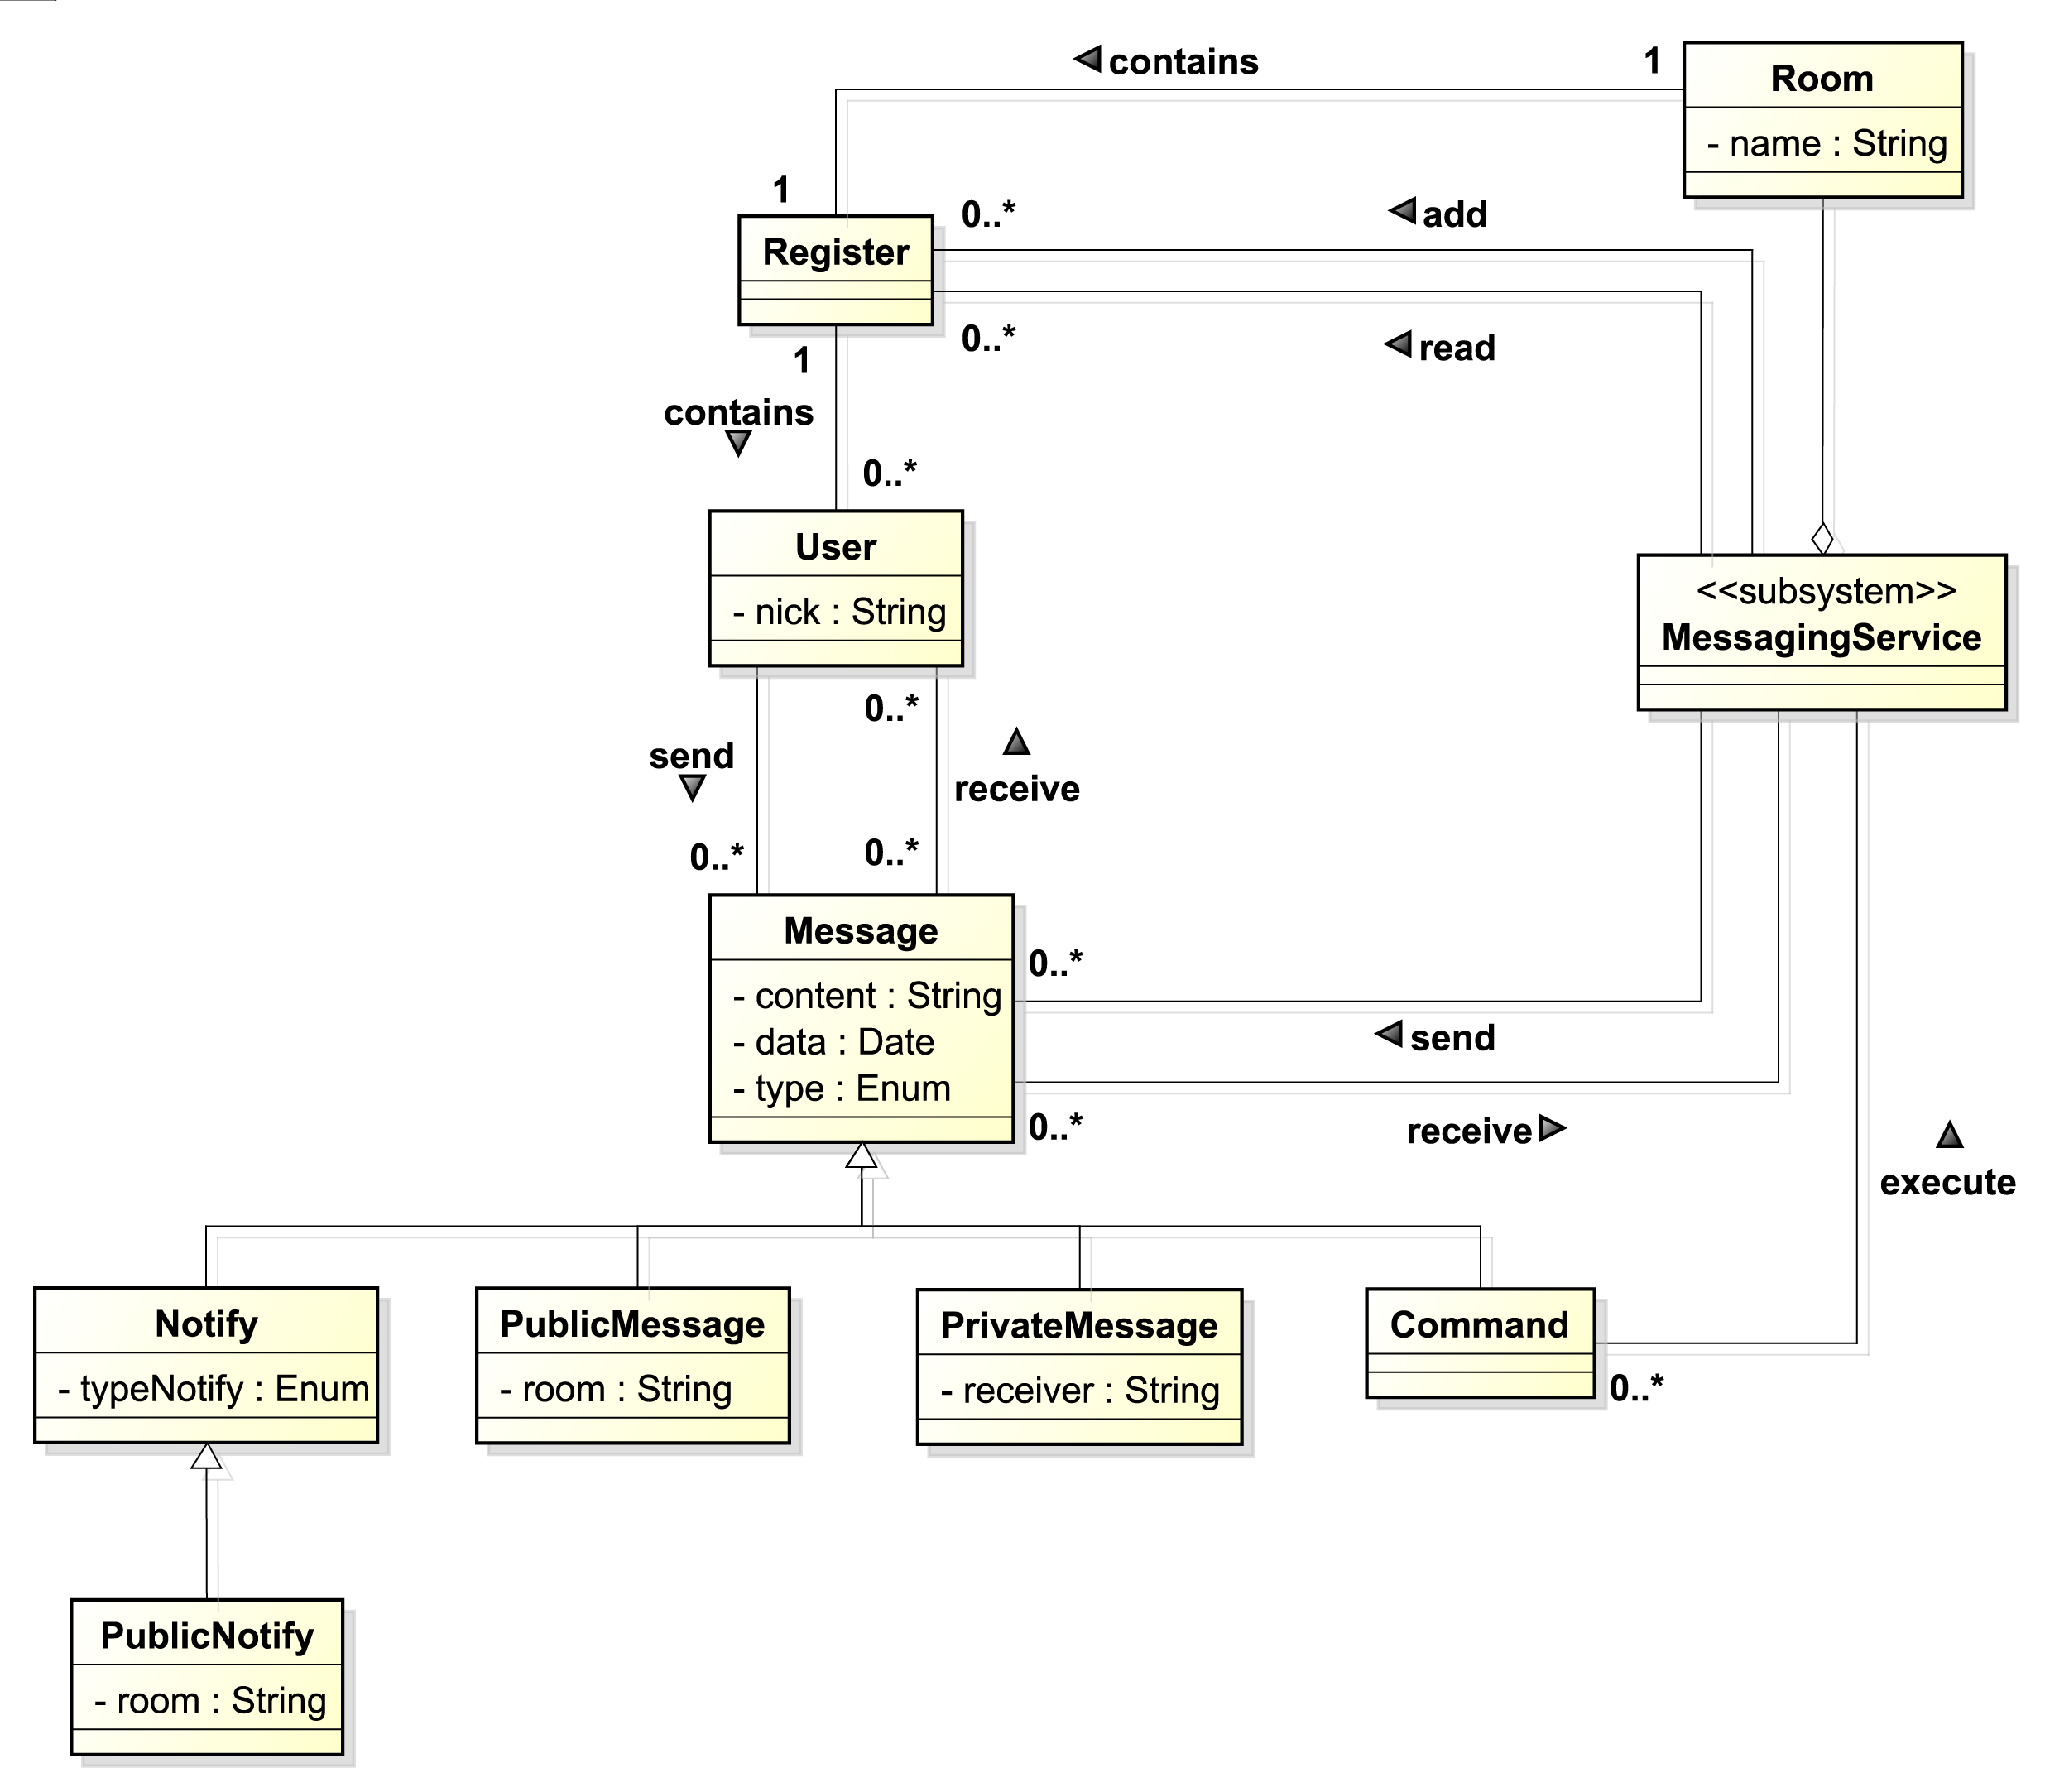
\includegraphics[scale=0.16]{image_astah/Iteration_3_DomainModel/UC4_SendPrivateMessage_DM.png}{\centering}
     \caption{UC3 - Modello di dominio}
     \label{fig_UC4_SPM_DM} 
   \end{figure}
\end{frame}

\begin{frame} {Iterazione 3: Analisi - UC4\_SendPrivateMessage}
   \begin{figure}
     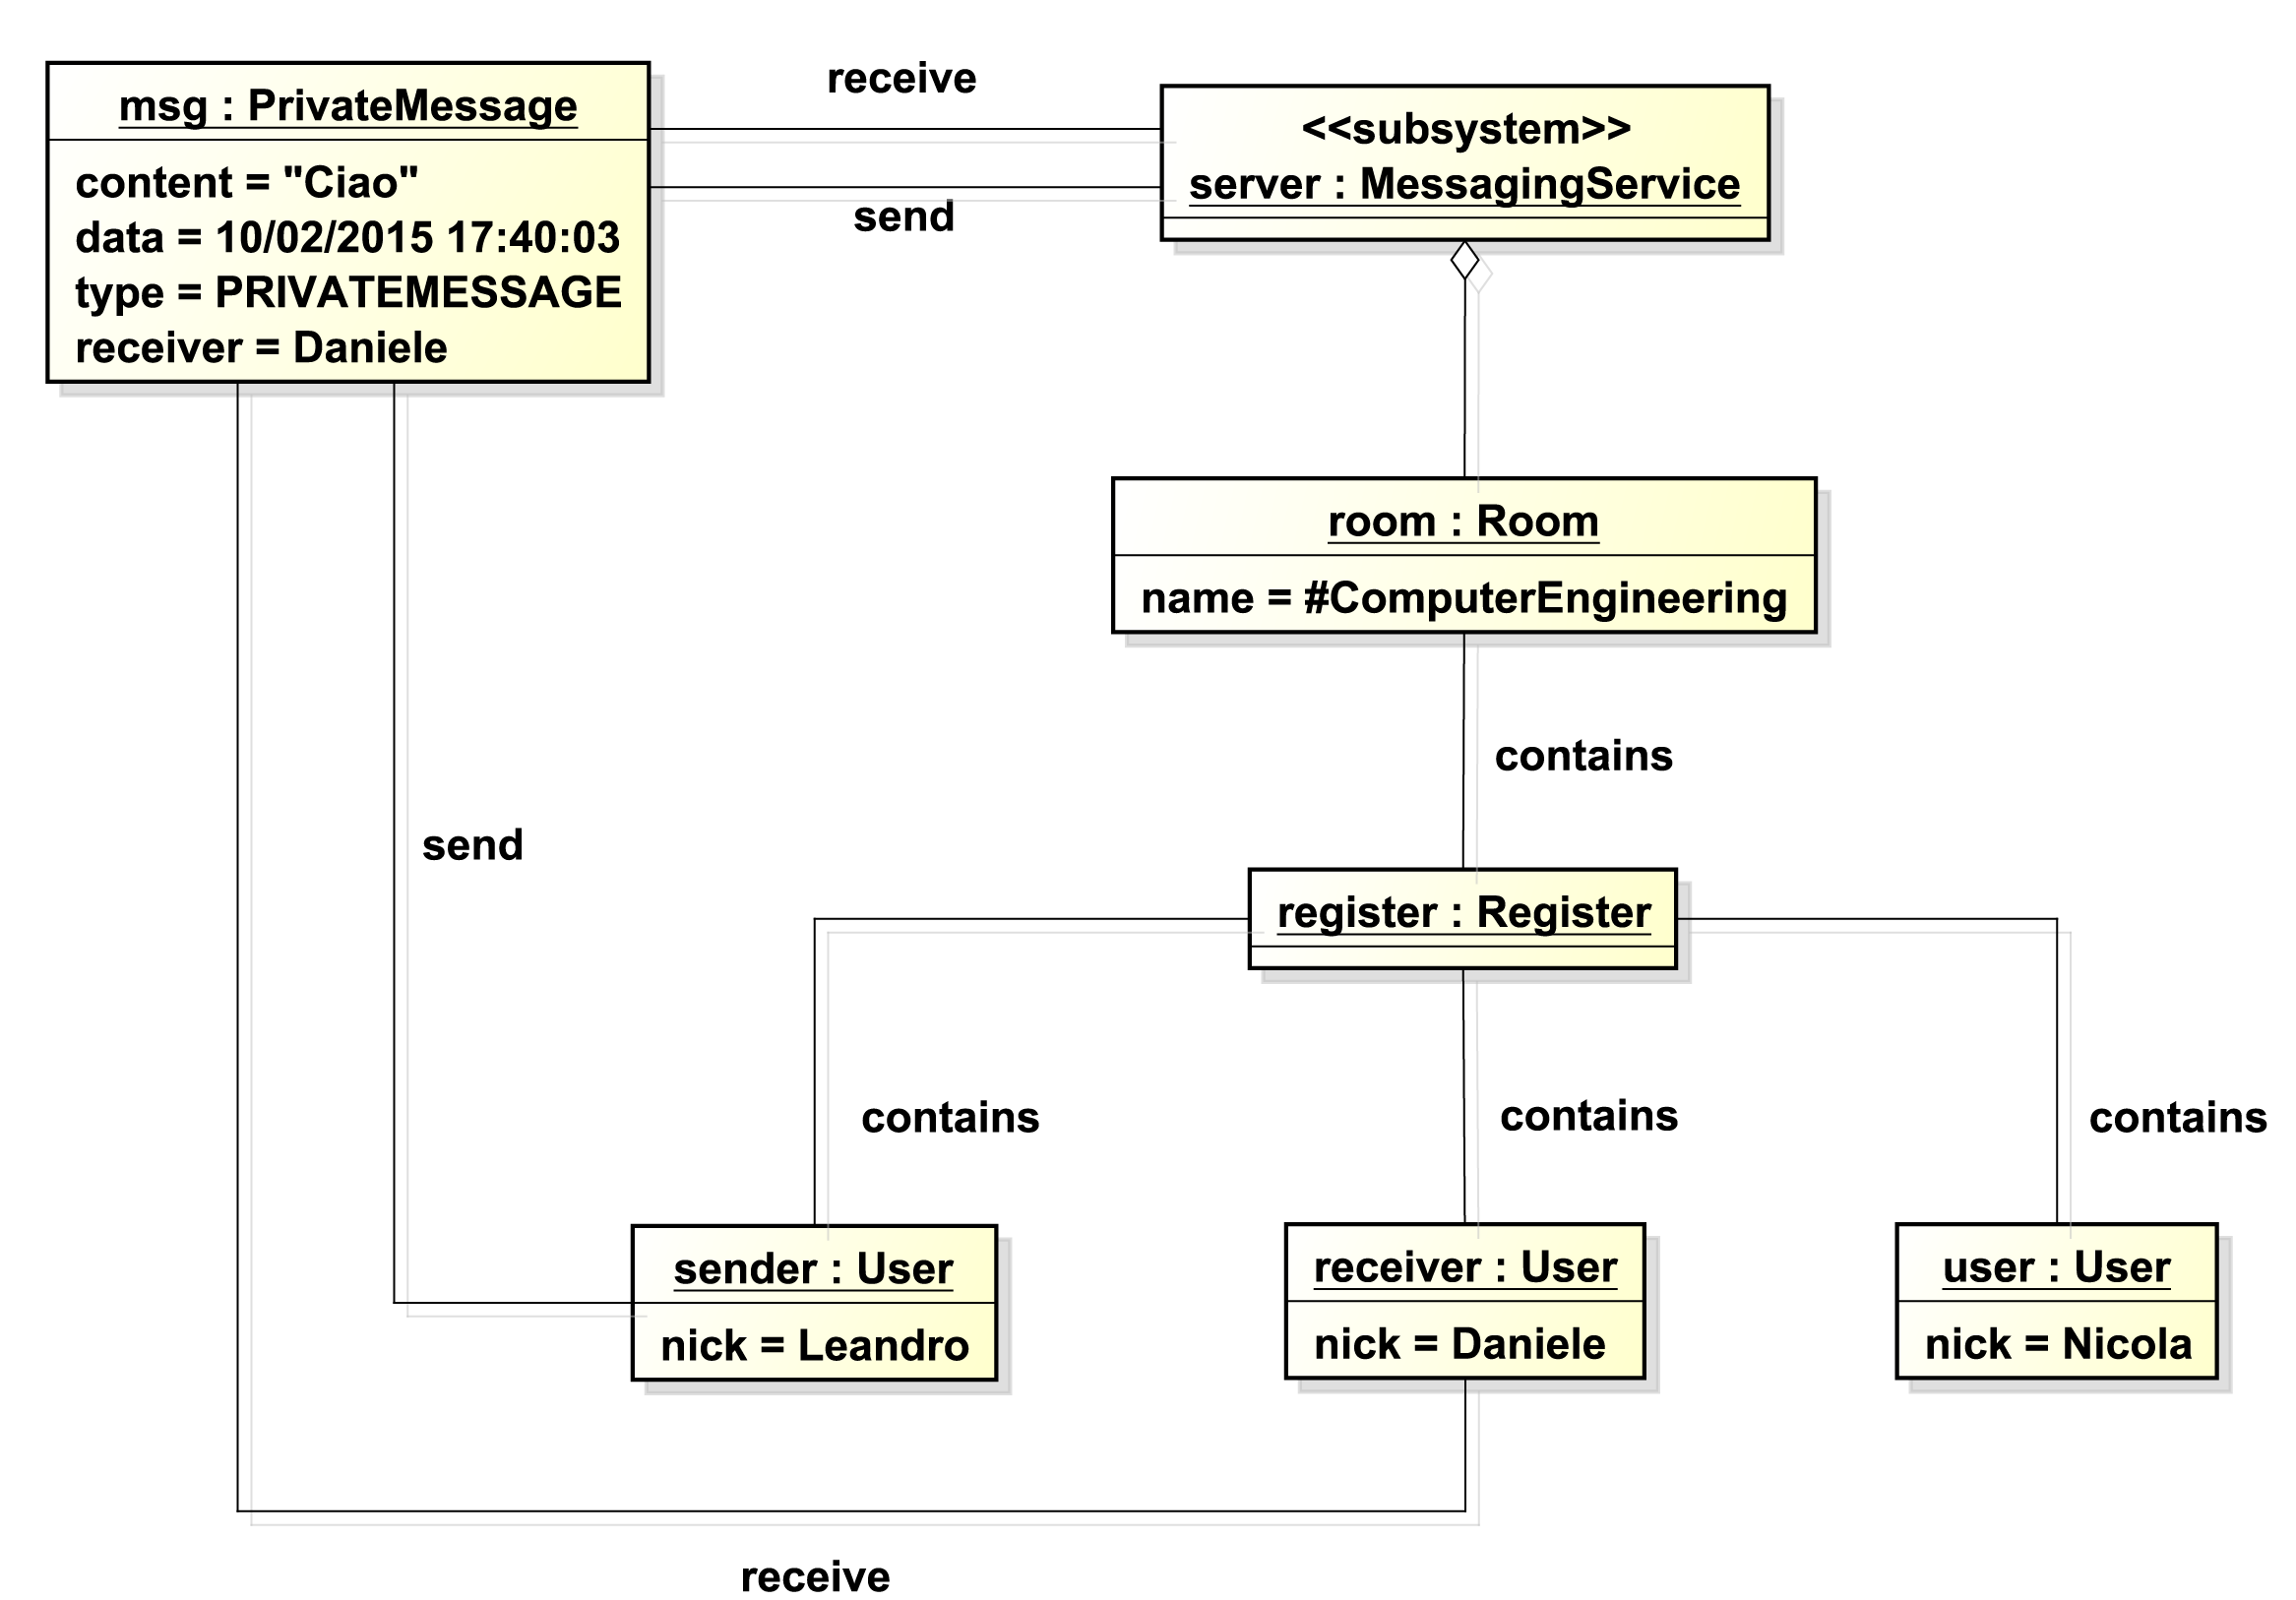
\includegraphics[scale=0.22]{image_astah/Iteration_3_DomainModel/UC4_SendPrivateMessage_OM.png}{\centering}
     \caption{UC3 - Oggetti di dominio}
     \label{fig_UC4_SPM_OM} 
   \end{figure}
\end{frame}

\begin{frame} {Iterazione 3: Analisi - UC4\_SendPrivateMessage}
   \begin{figure}
     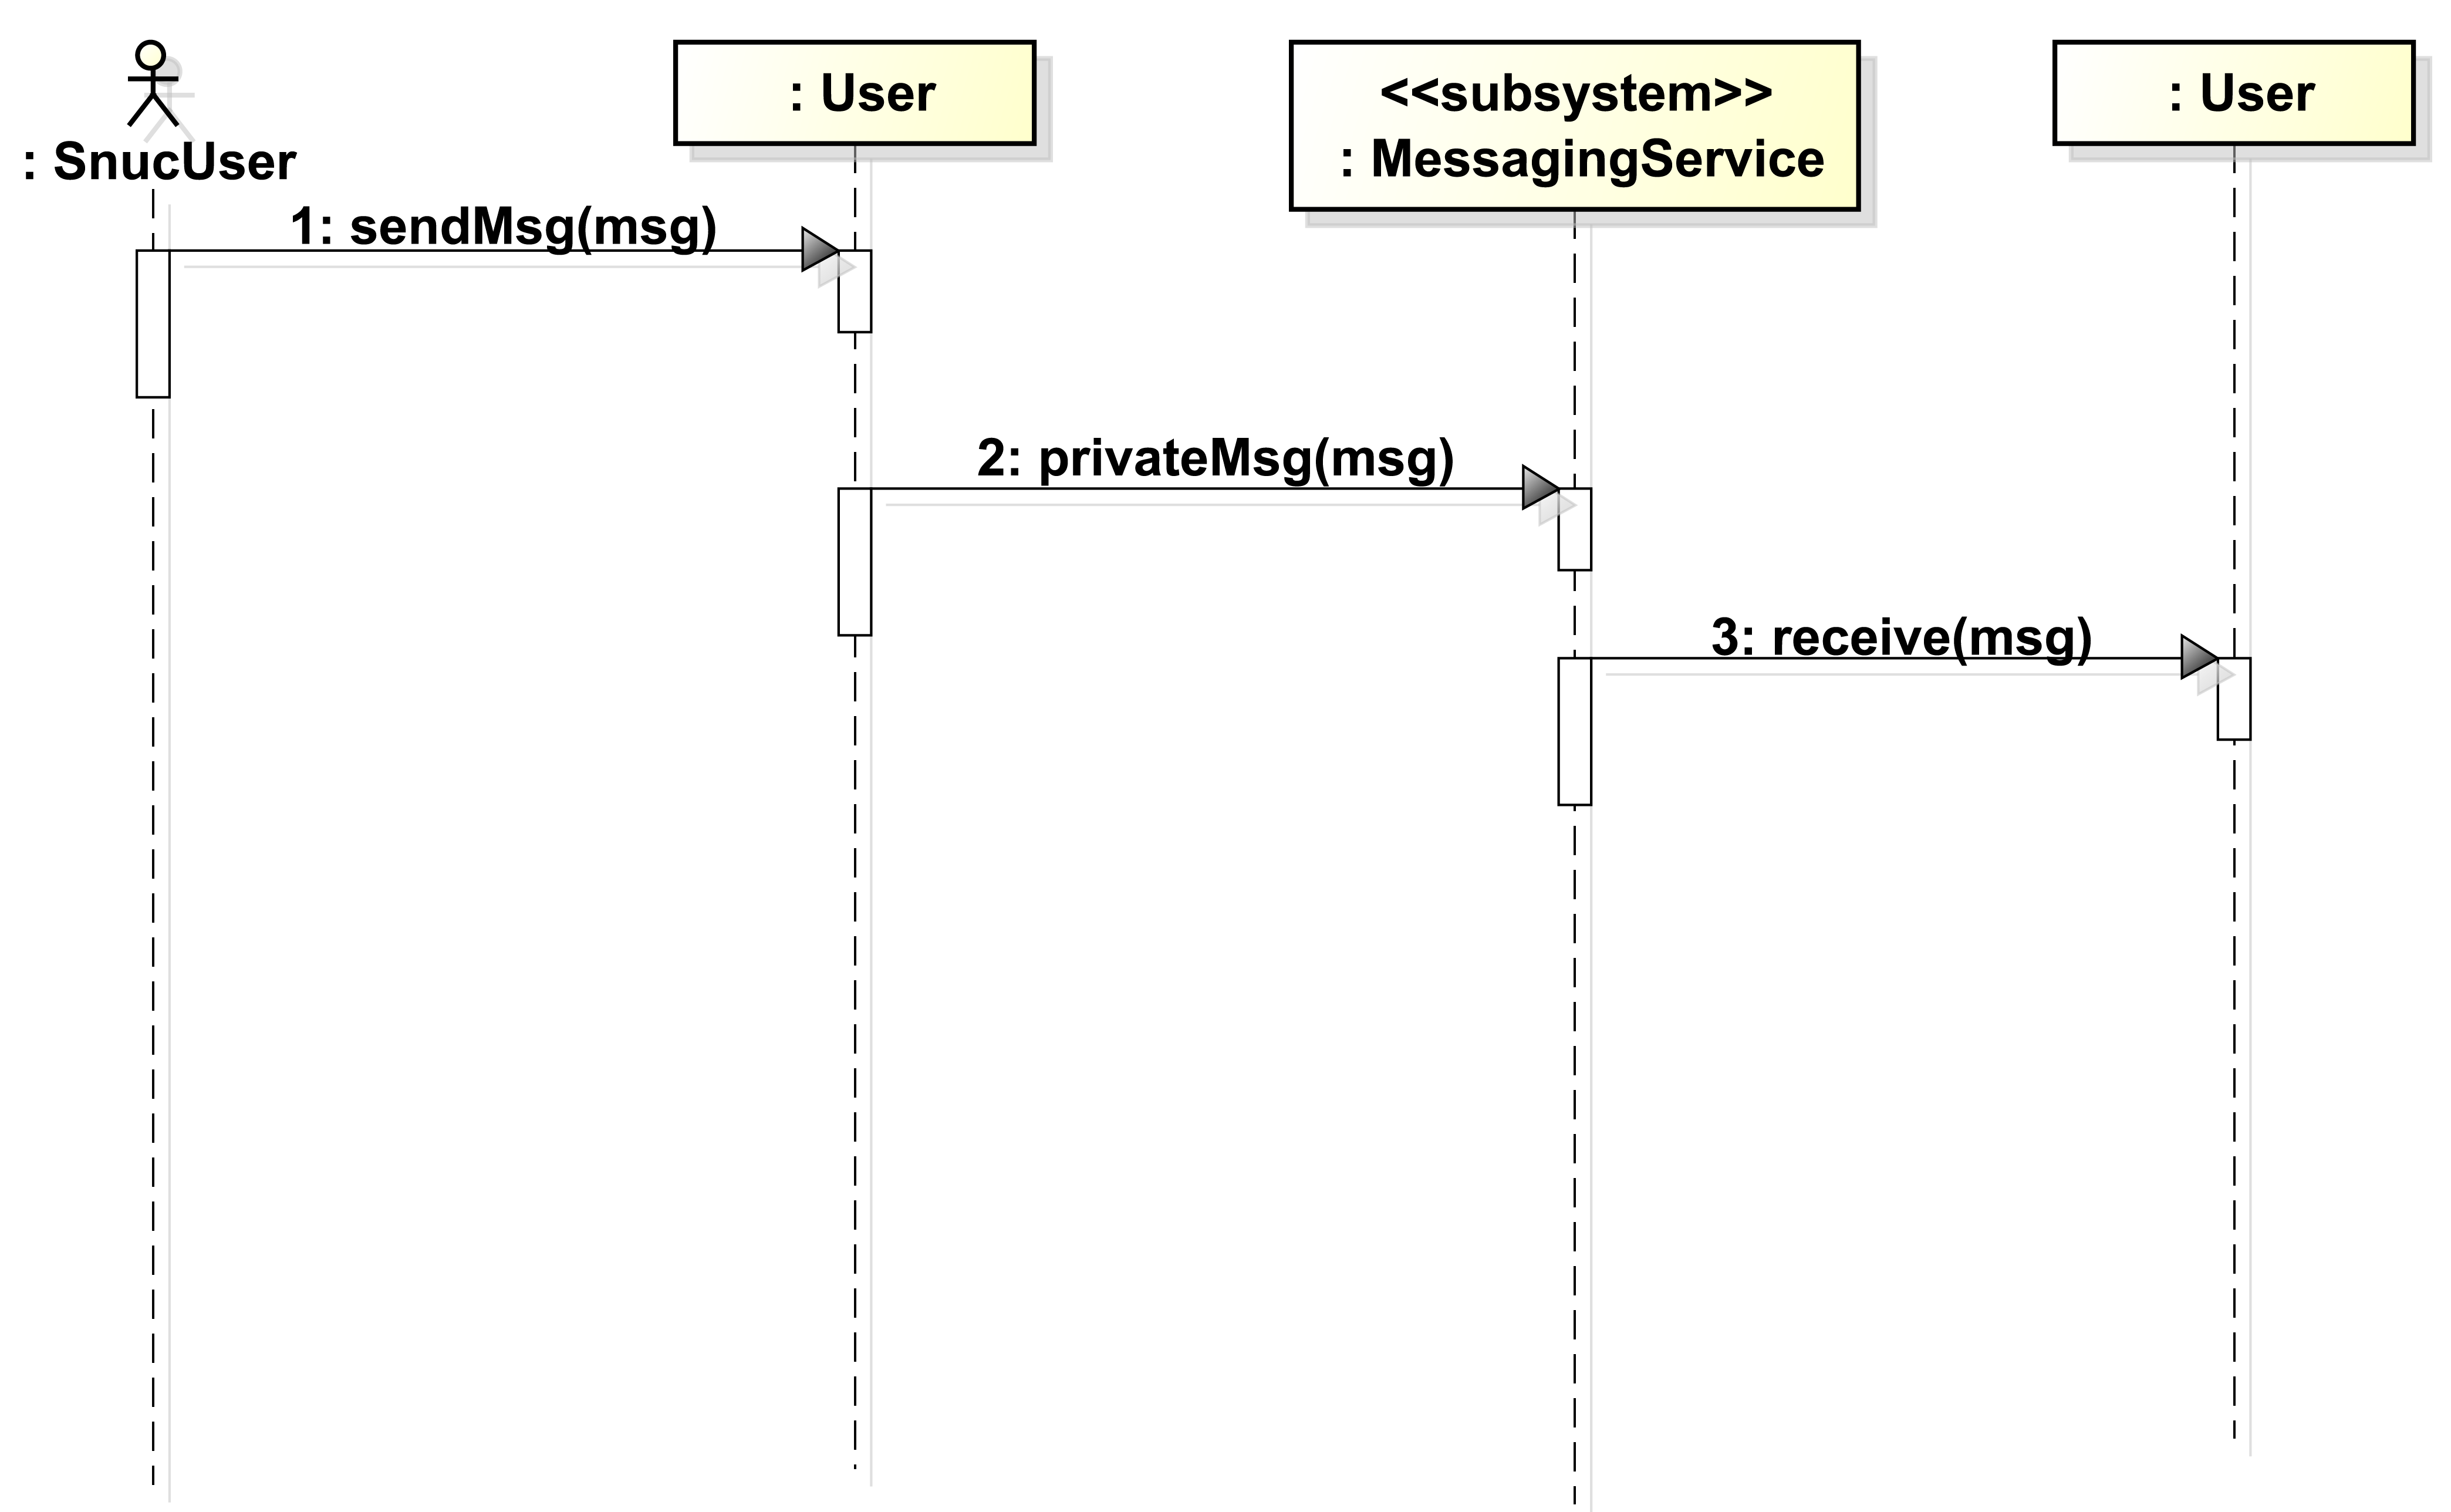
\includegraphics[scale=0.28]{image_astah/Iteration_3_DomainModel/UC4_SendPrivateMessage_SSD.png}{\centering}
     \caption{UC4 - Diagramma di sequenza di sistema}
     \label{fig_UC4_SPM_SSD} 
   \end{figure}
\end{frame}

\begin{frame}
 \frametitle{Iterazione 3: Analisi, UC4 contratto CO6 }
  \begin{table}[!htbp]
   \caption {UC3 Contratto CO6 - privateMsg}
    \label{table_CO6}
      \resizebox{\linewidth}{!}{%
       \begin{tabular}{|l|p{10cm}|}\hline
         Operazione & \textit{privateMsg(msg:PublicMessage)} \\\hline 
         Riferimenti & Caso d’uso: UC4\_SendPrivateMessage \\\hline
         Pre-condizione & 
         \begin{itemize}
          \item L'utente è registrato nella stanza
          \item L'utente seleziona il destinatario del messaggio privato tra gli utenti registrati nella stanza    
         \end{itemize} \\\hline 
         Post-condizione & Il destinatario riceve il messaggio privato  \\\hline
      \end{tabular}}
   \end{table}
\end{frame}

\subsection{Iterazione 3: Progettazione}
\begin{frame} {Descrizione Iterazione 3: Progettazione}
  \emph{INSERIRE DESCRIZIONE}
\end{frame}

\subsection{Iterazione 3: Progettazione Class Diagram UC4}
\begin{frame} {Iterazione 3: Progettazione Class Diagram Common UC4}
   \begin{figure}
     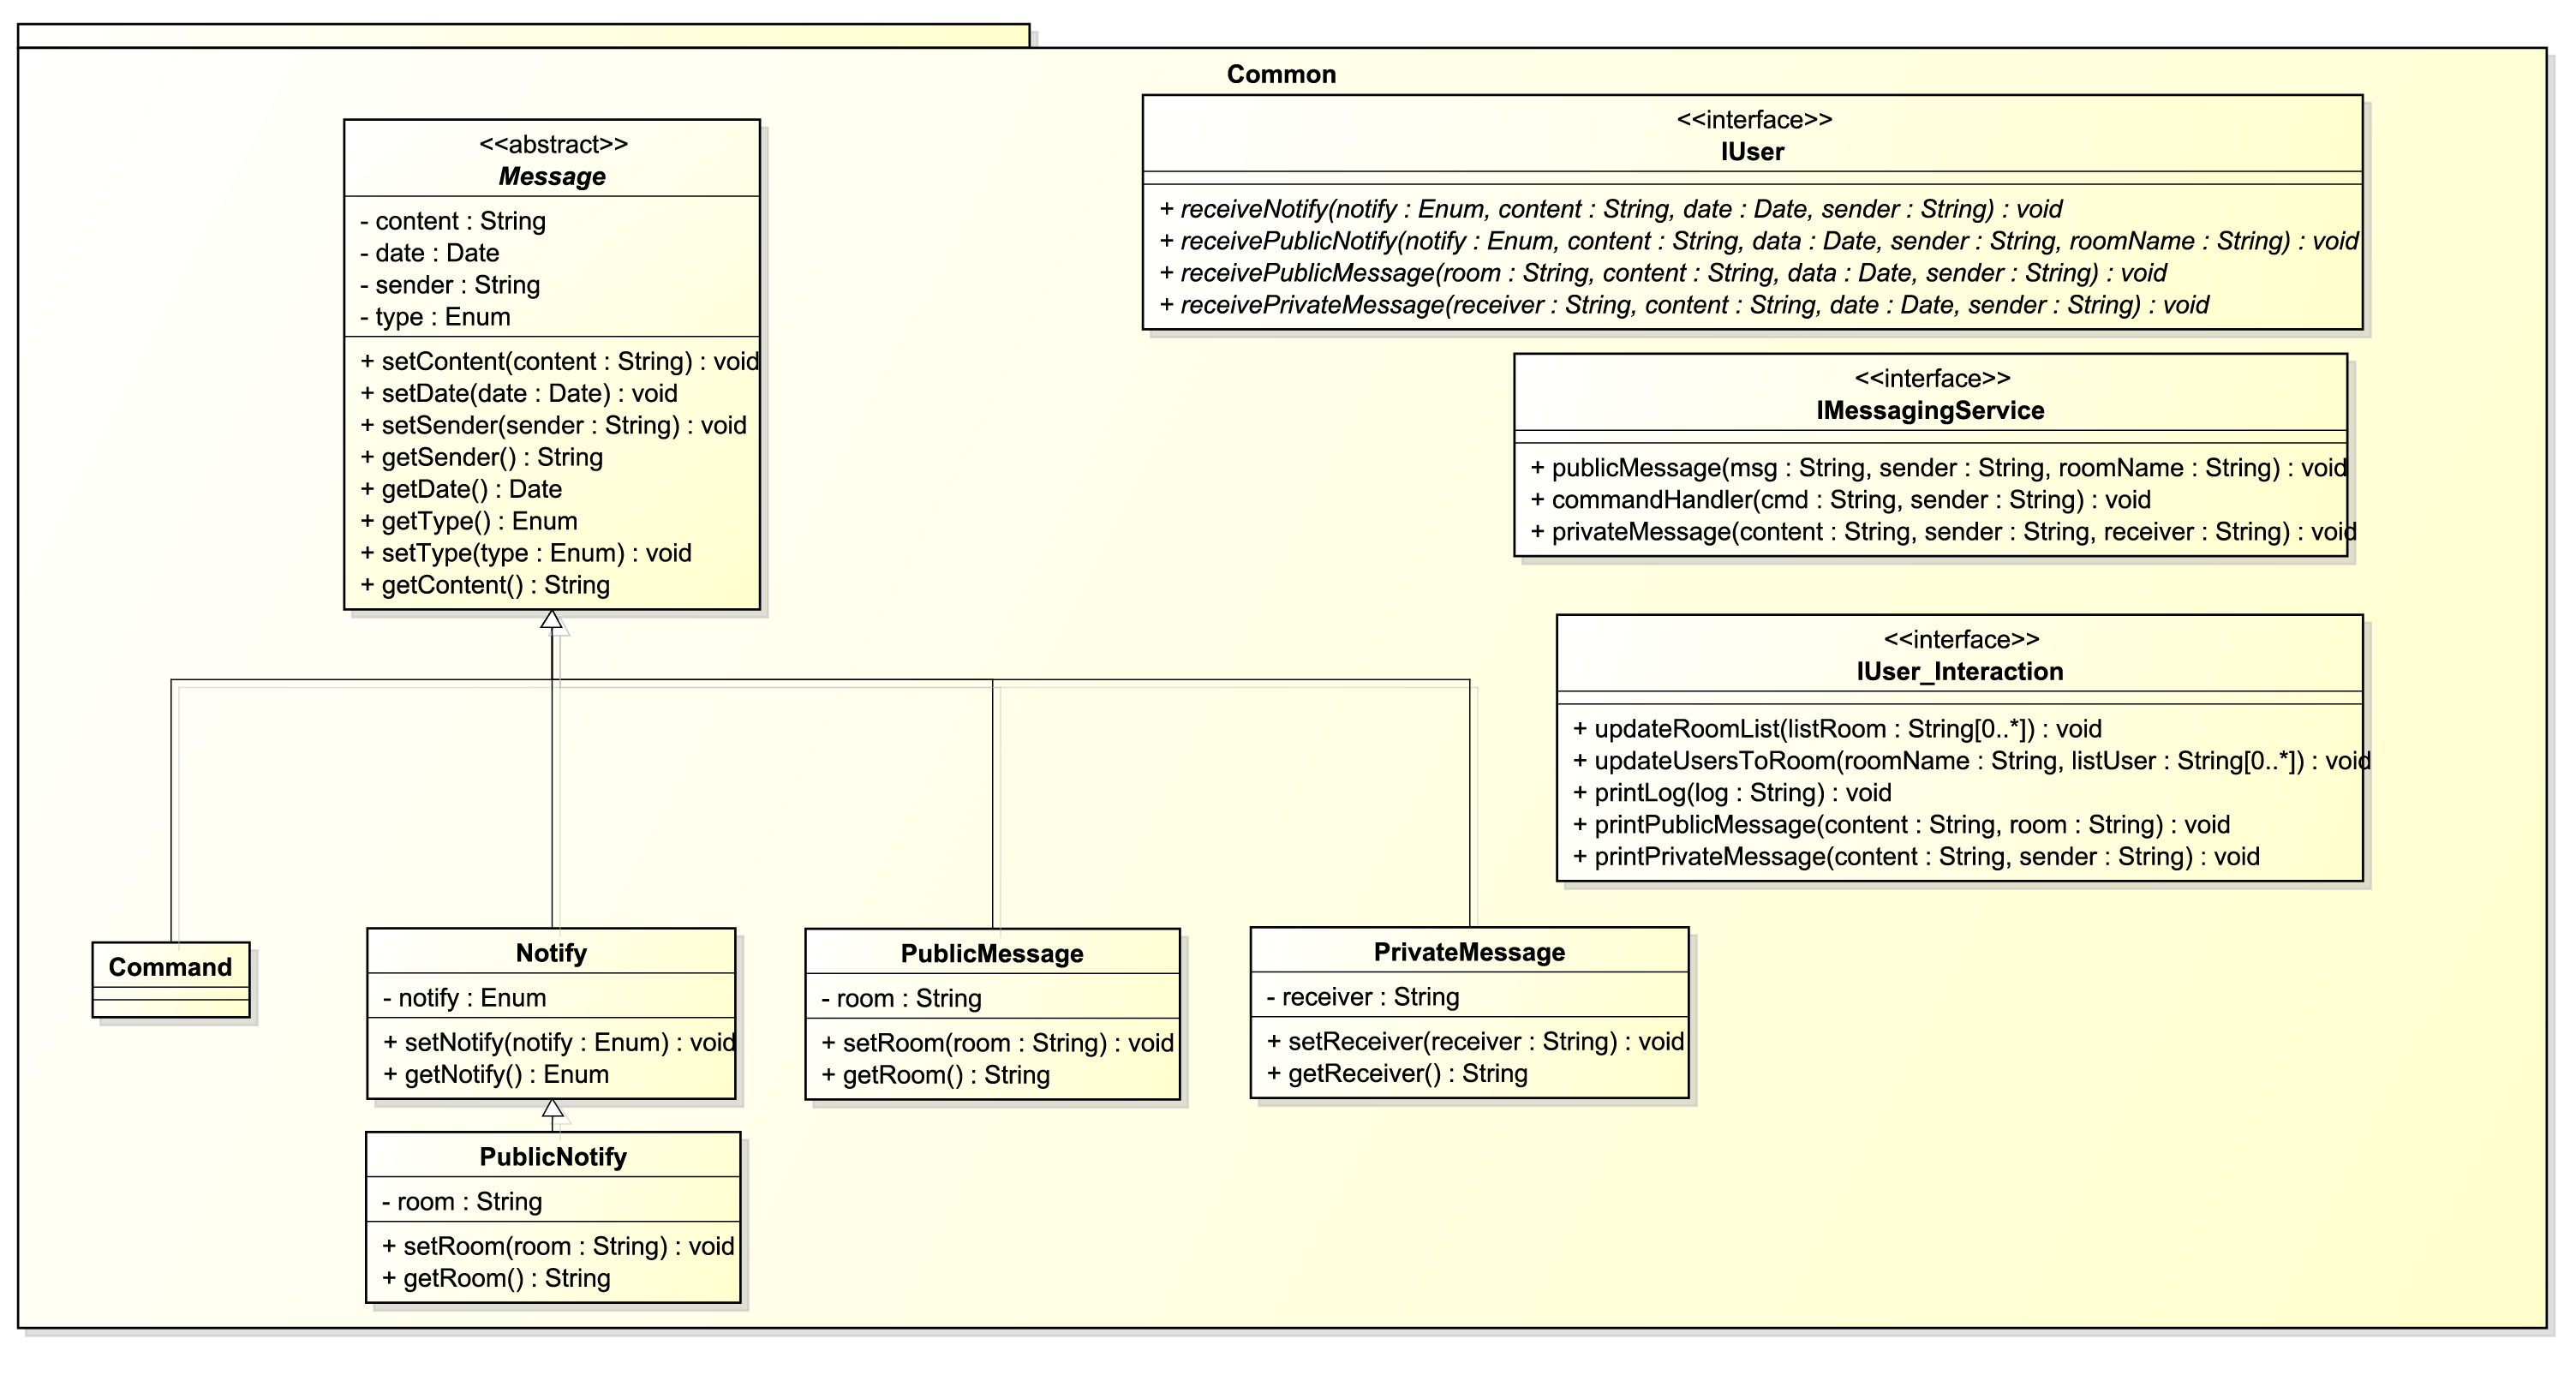
\includegraphics[scale=0.15]{image_astah/Iteration_3_DesignModel/ClassDiagramCommon.png}{\centering}
     \caption{DCD - Diagramma delle Classi: Package Common }
     \label{fig_UC4_DCD_1} 
   \end{figure}
\end{frame}

\begin{frame} {Iterazione 3: Progettazione Class Diagram Snuc UC4}
   \begin{figure}
     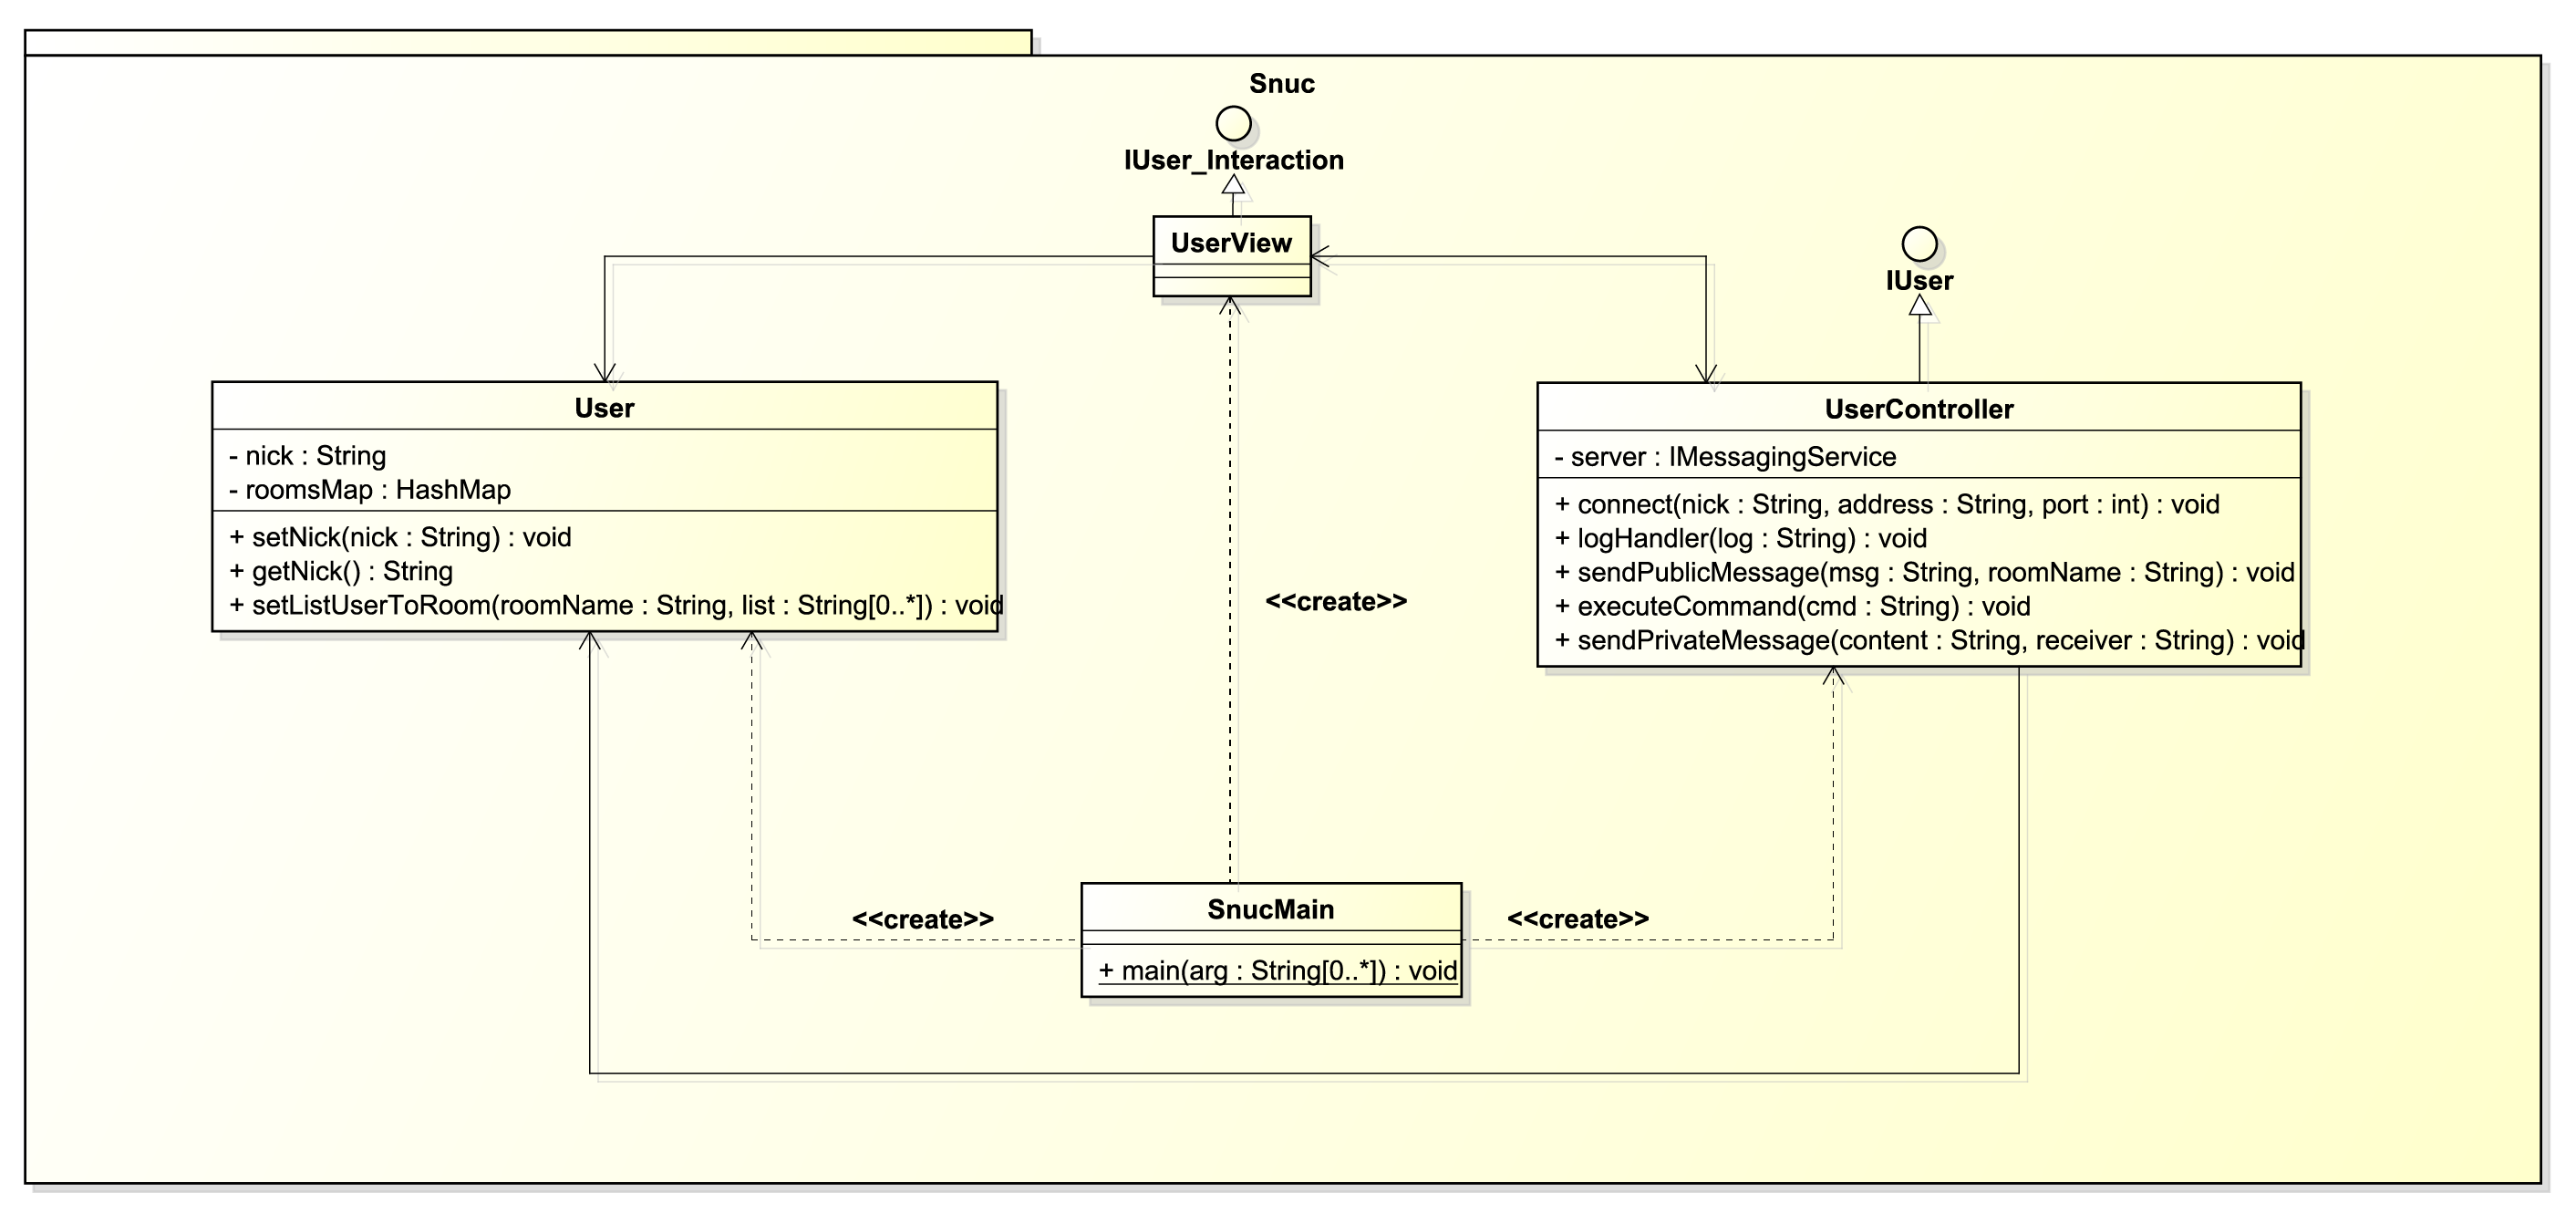
\includegraphics[scale=0.16]{image_astah/Iteration_3_DesignModel/ClassDiagramSnuc.png}{\centering}
     \caption{DCD - Diagramma delle Classi: Package Snuc }
     \label{fig_UC4_DCD_3} 
   \end{figure}
\end{frame}

\begin{frame} {Iterazione 3: Progettazione Class Diagram Connector UC4}
   \begin{figure}
     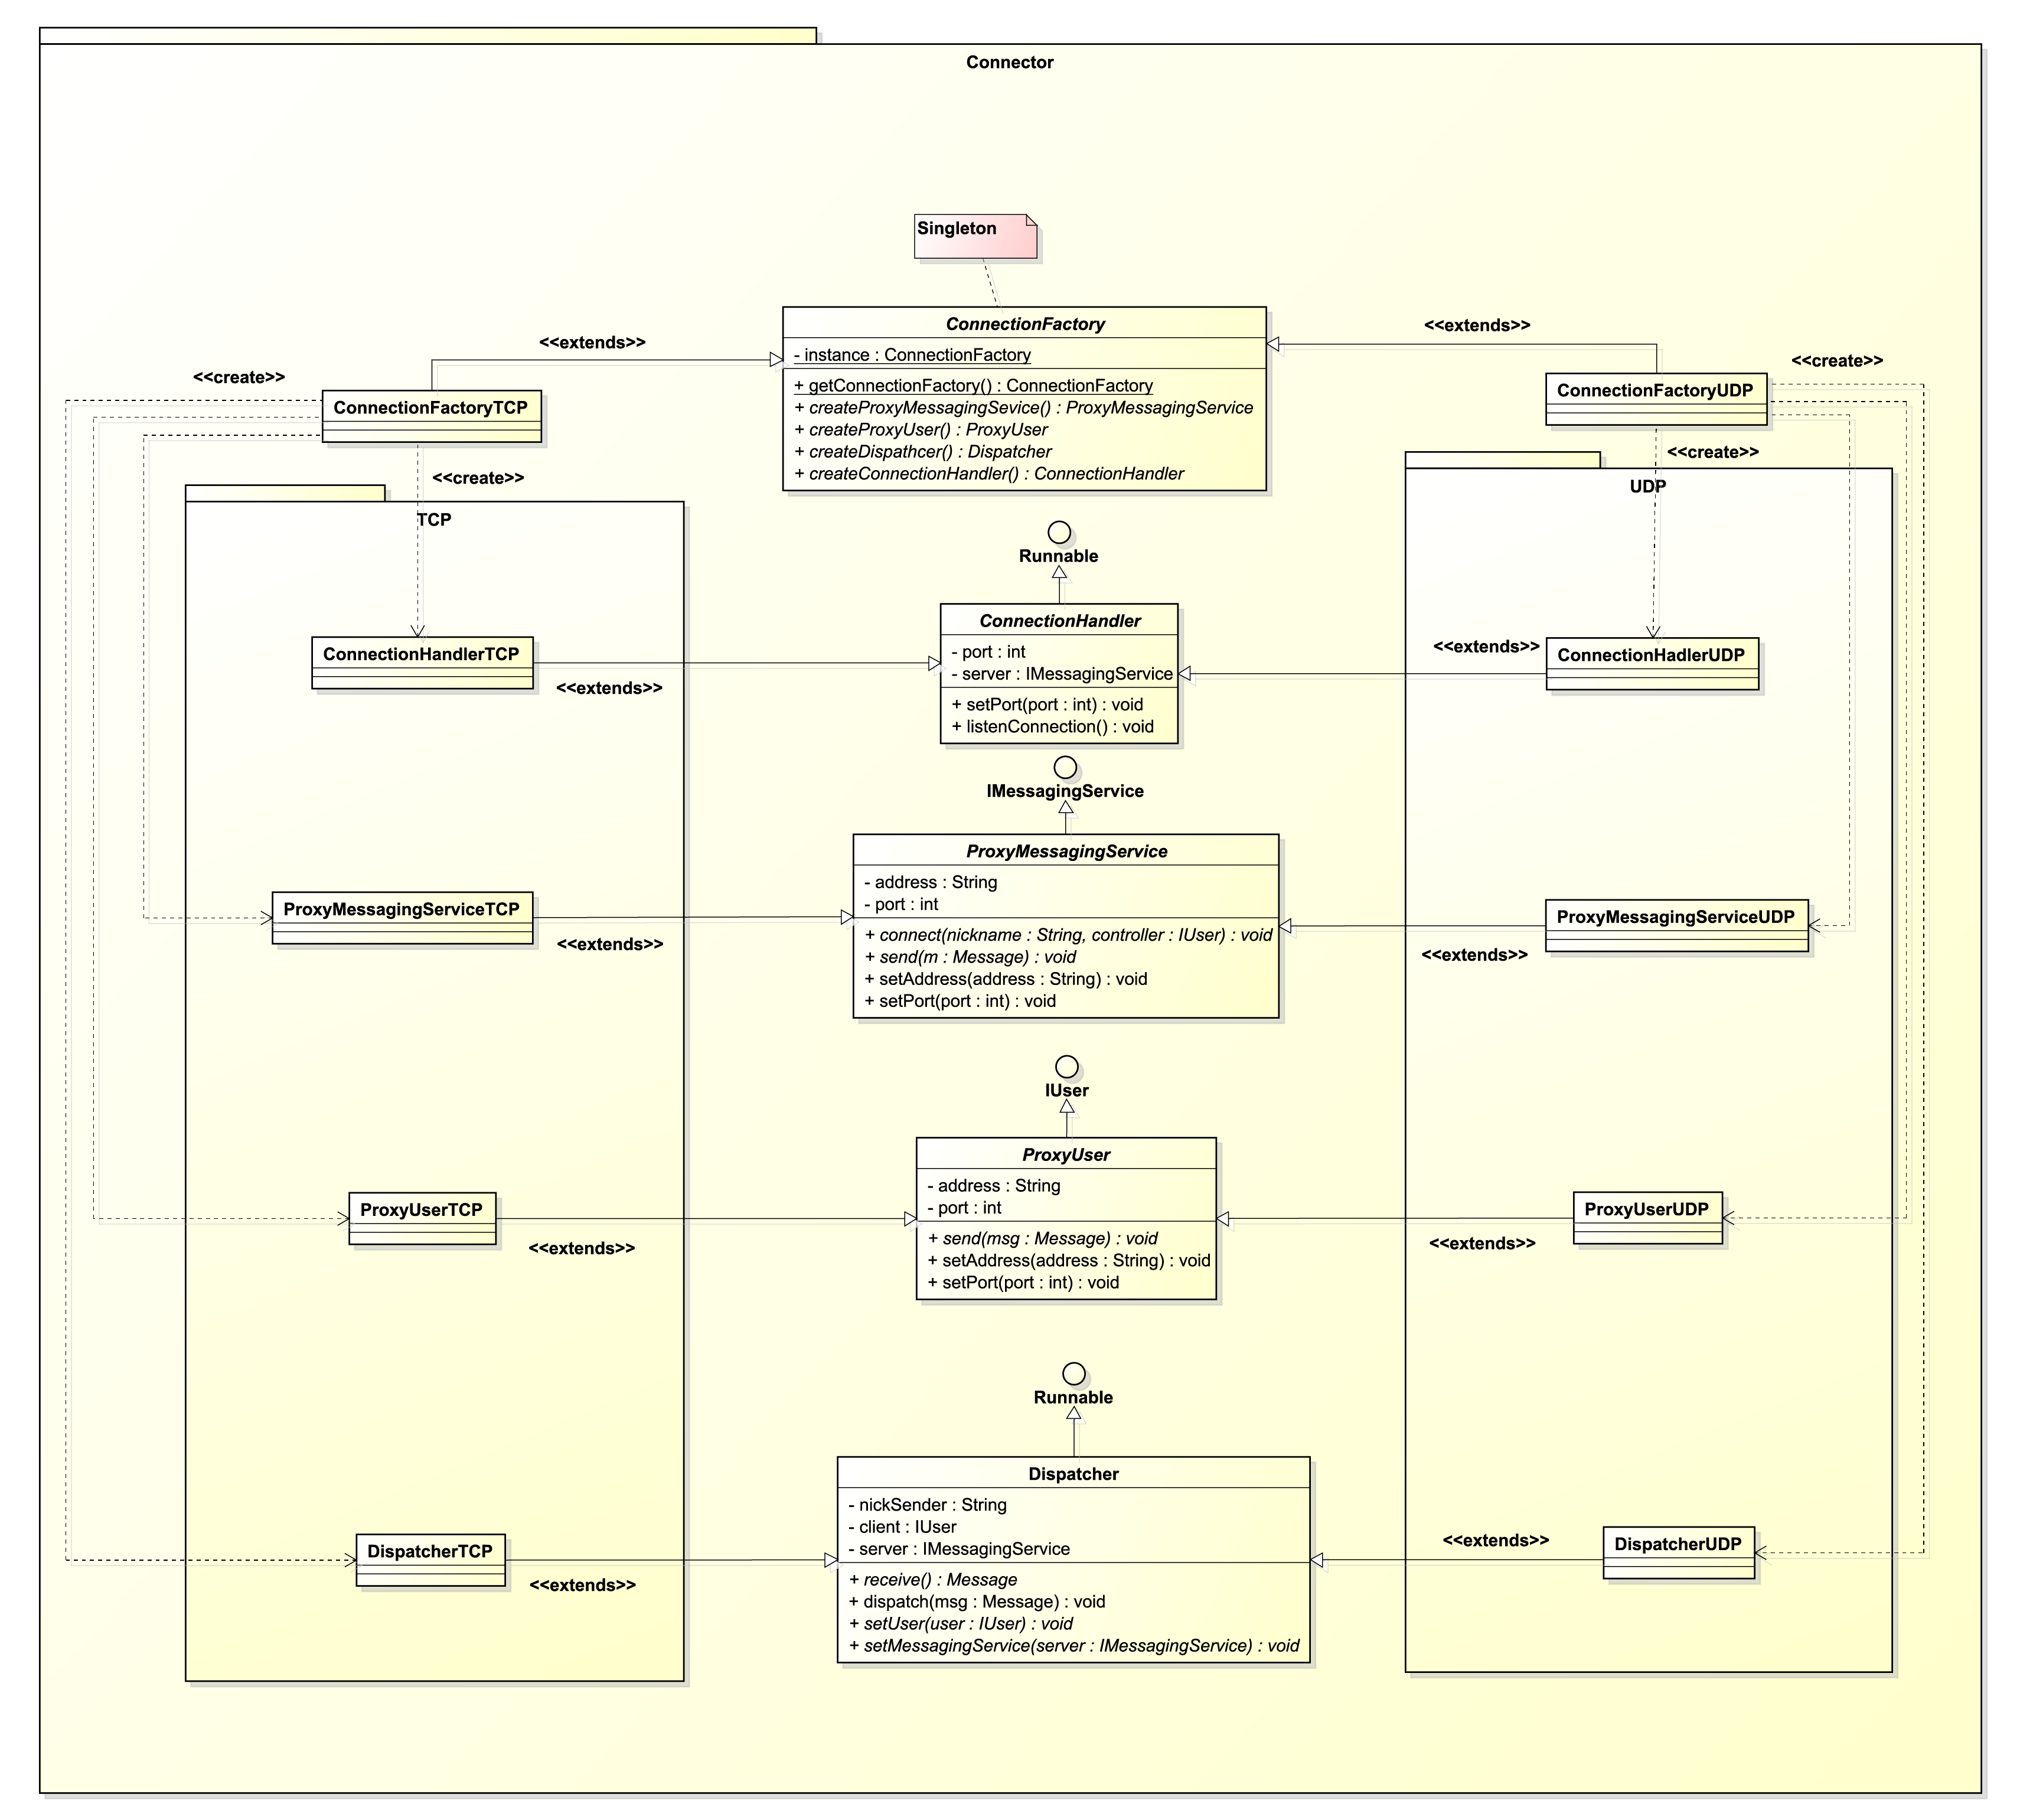
\includegraphics[scale=0.077]{image_astah/Iteration_3_DesignModel/ClassDiagramConnector.png}{\centering}
     \caption{DCD - Diagramma delle Classi: Package Connector }
     \label{fig_UC4_DCD_4} 
   \end{figure}
\end{frame}

\begin{frame} {Iterazione 3: Progettazione Class Diagram Snuc Server UC4}
   \begin{figure}
     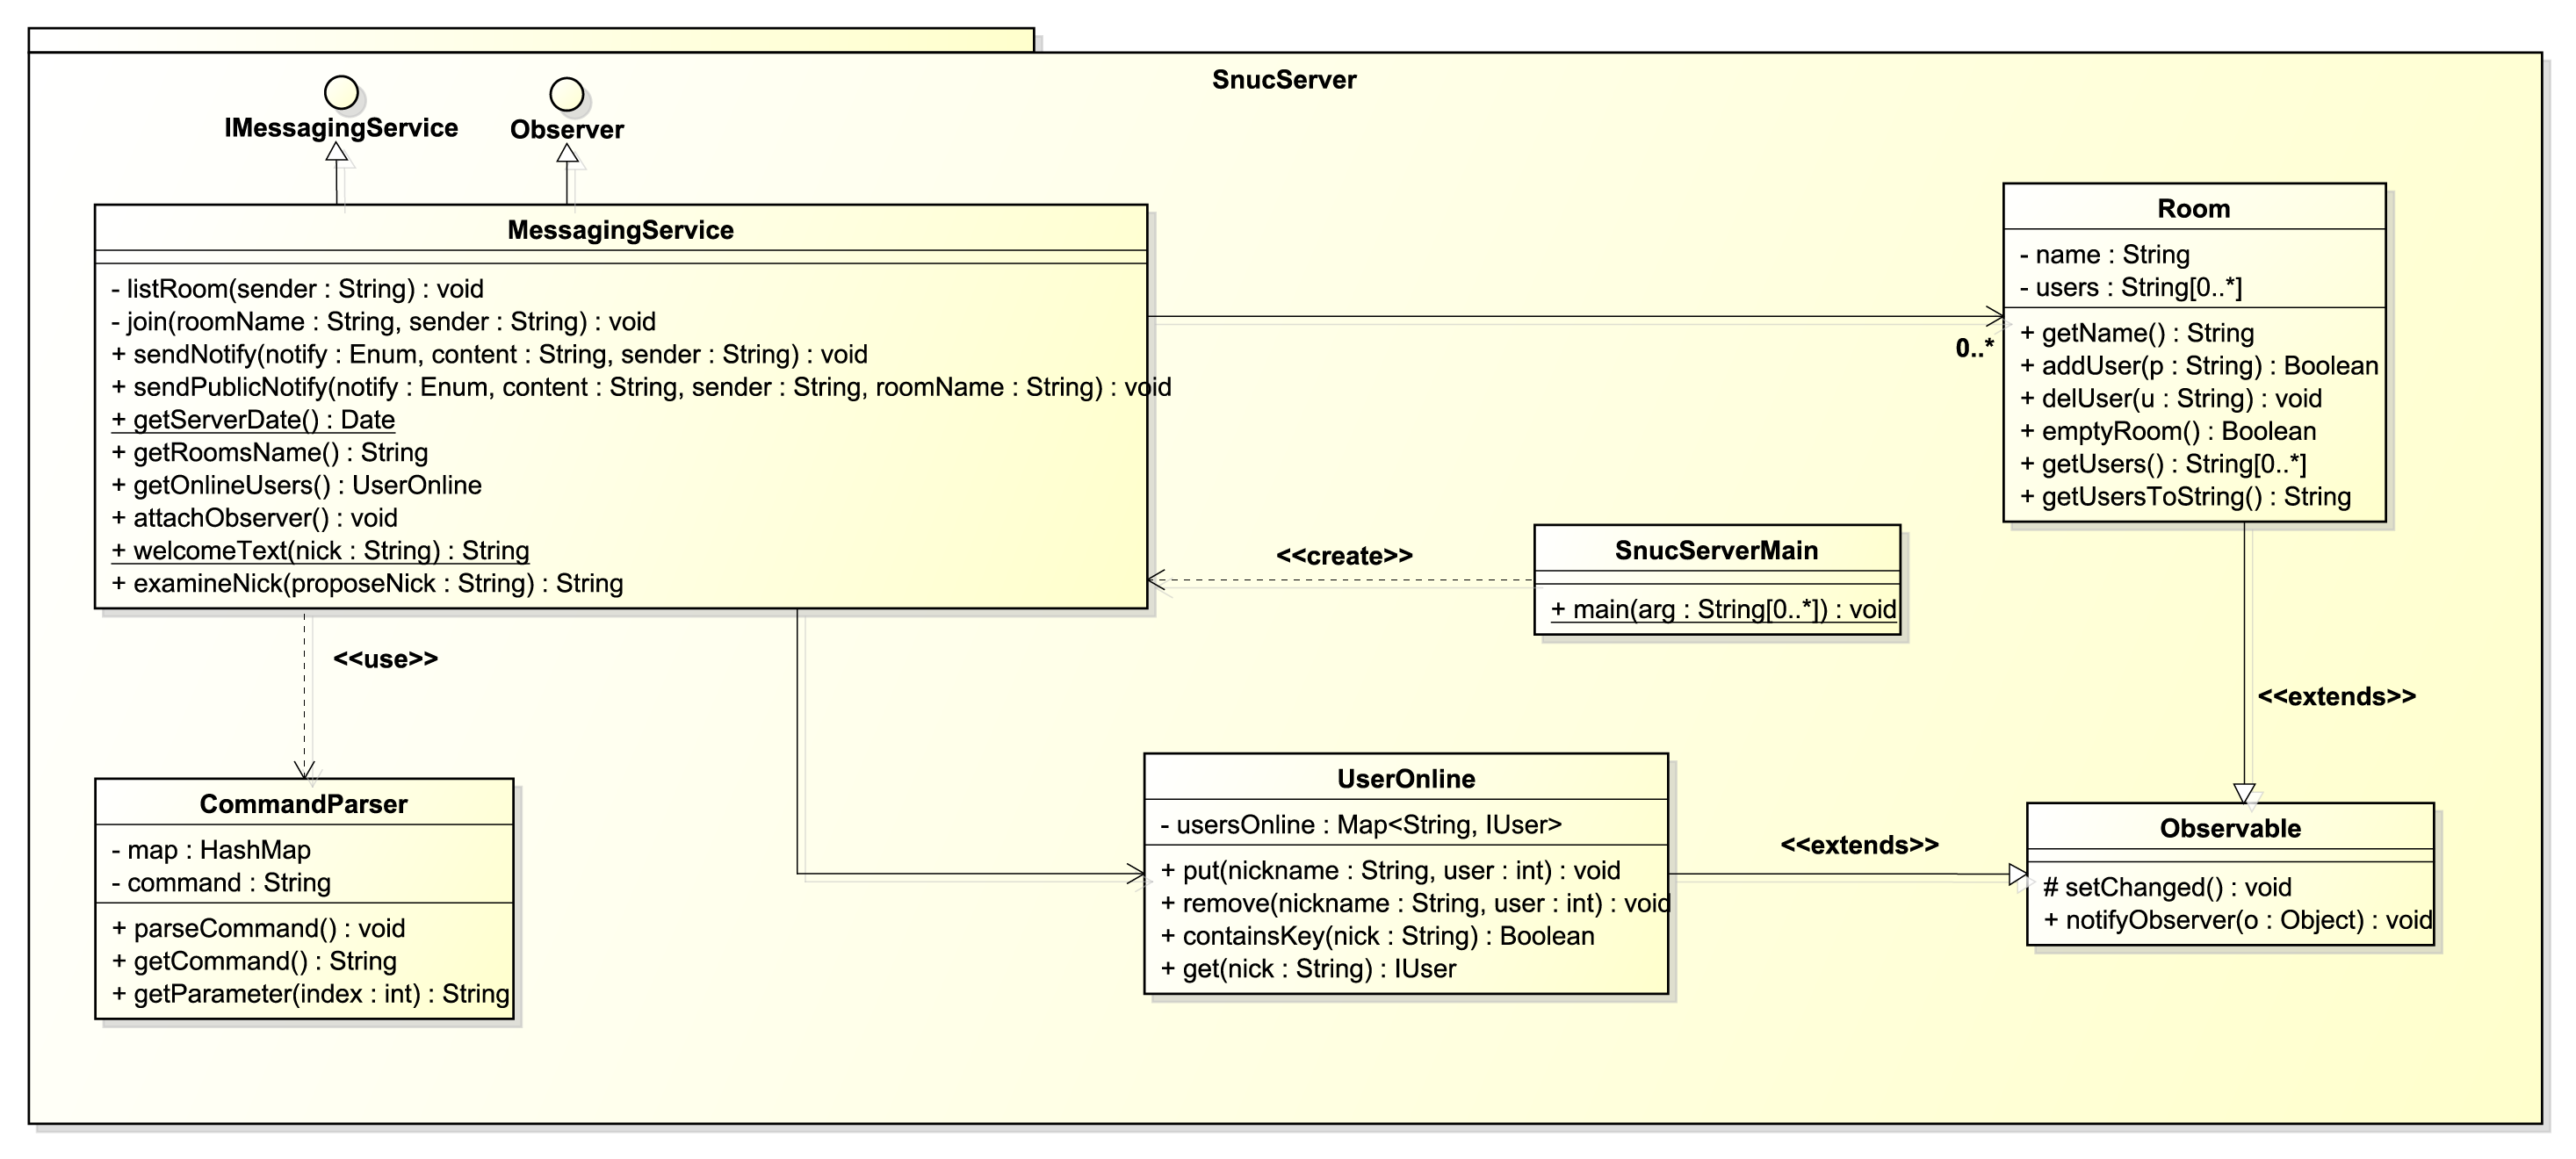
\includegraphics[scale=0.155]{image_astah/Iteration_3_DesignModel/ClassDiagramSnucServer.png}{\centering}
     \caption{DCD - Diagramma delle Classi: Package Snuc Server }
     \label{fig_UC4_DCD_2} 
   \end{figure}
\end{frame}

\subsection{Iterazione 3: Progettazione - SSD UC4\_SendPrivateMessage}
\begin{frame} {Iterazione 3: Progettazione, UC4\_SendPrivateMessage - OP1}
   \begin{figure}
     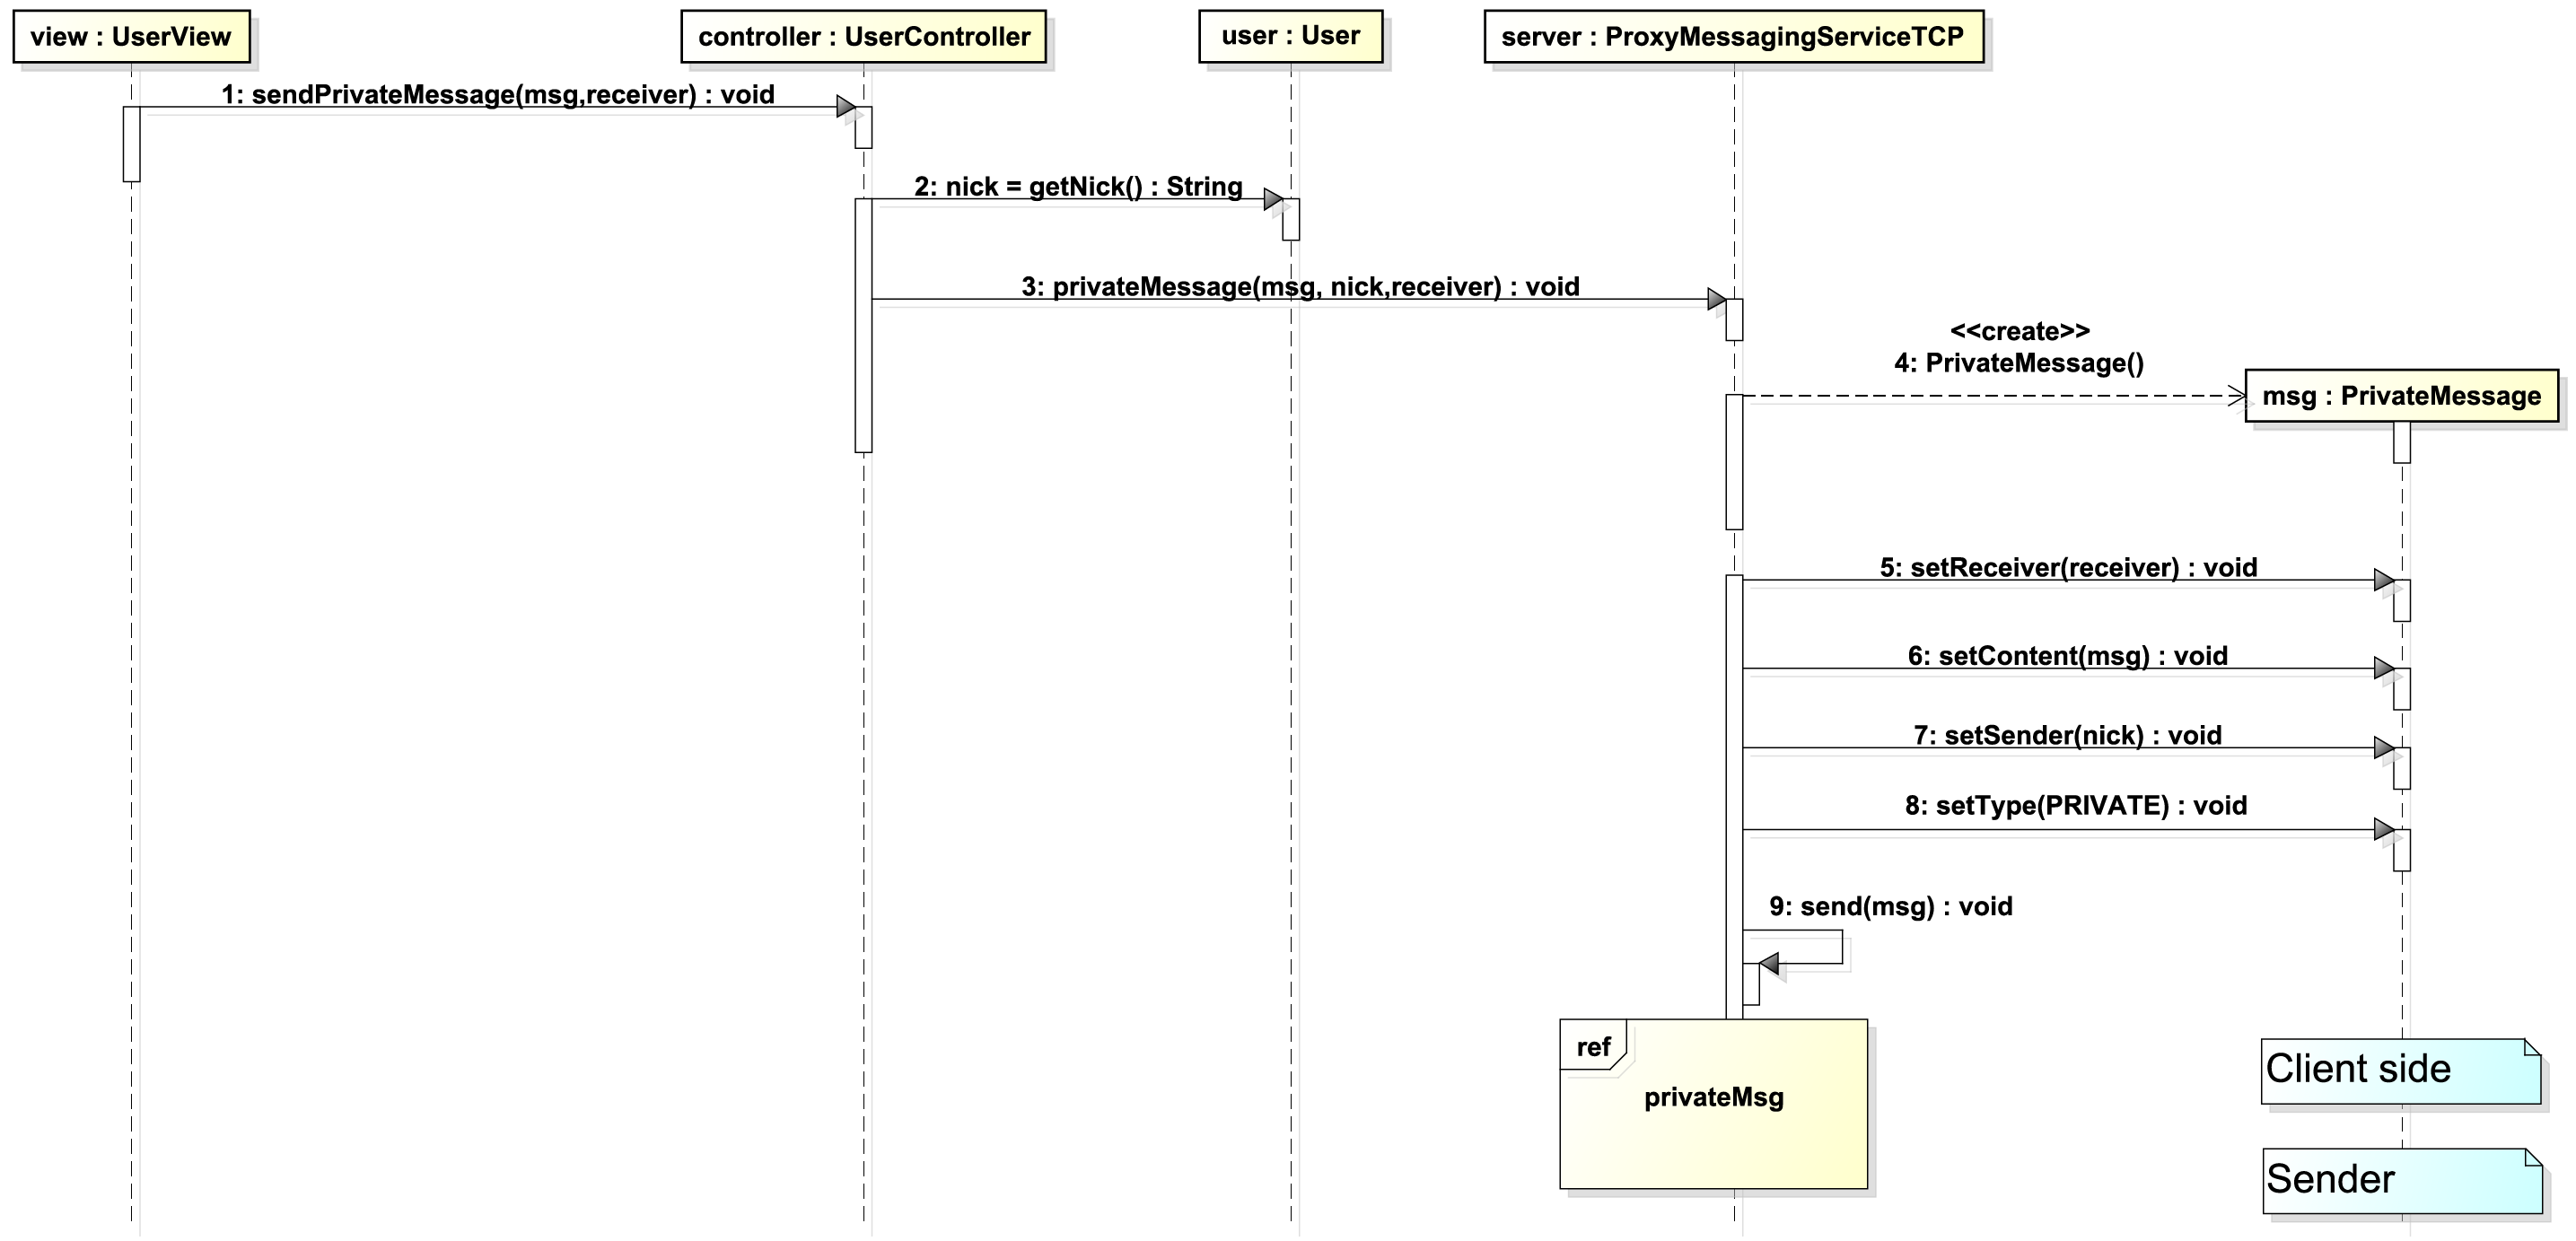
\includegraphics[scale=0.16]{image_astah/Iteration_3_DesignModel/UC4_SendPrivateMessage_SSD_1_sendMsg.png}{\centering}
     \caption{SSD - OP1: sendMsg(msg) del modello di dominio (figura \ref{fig_UC4_SPM_SSD}) }
     \label{fig_UC4_SSD_SRM_1} 
   \end{figure}
\end{frame}

\begin{frame} {Iterazione 3: Progettazione, UC4\_SendPrivateMessage - OP2}
   \begin{figure}
     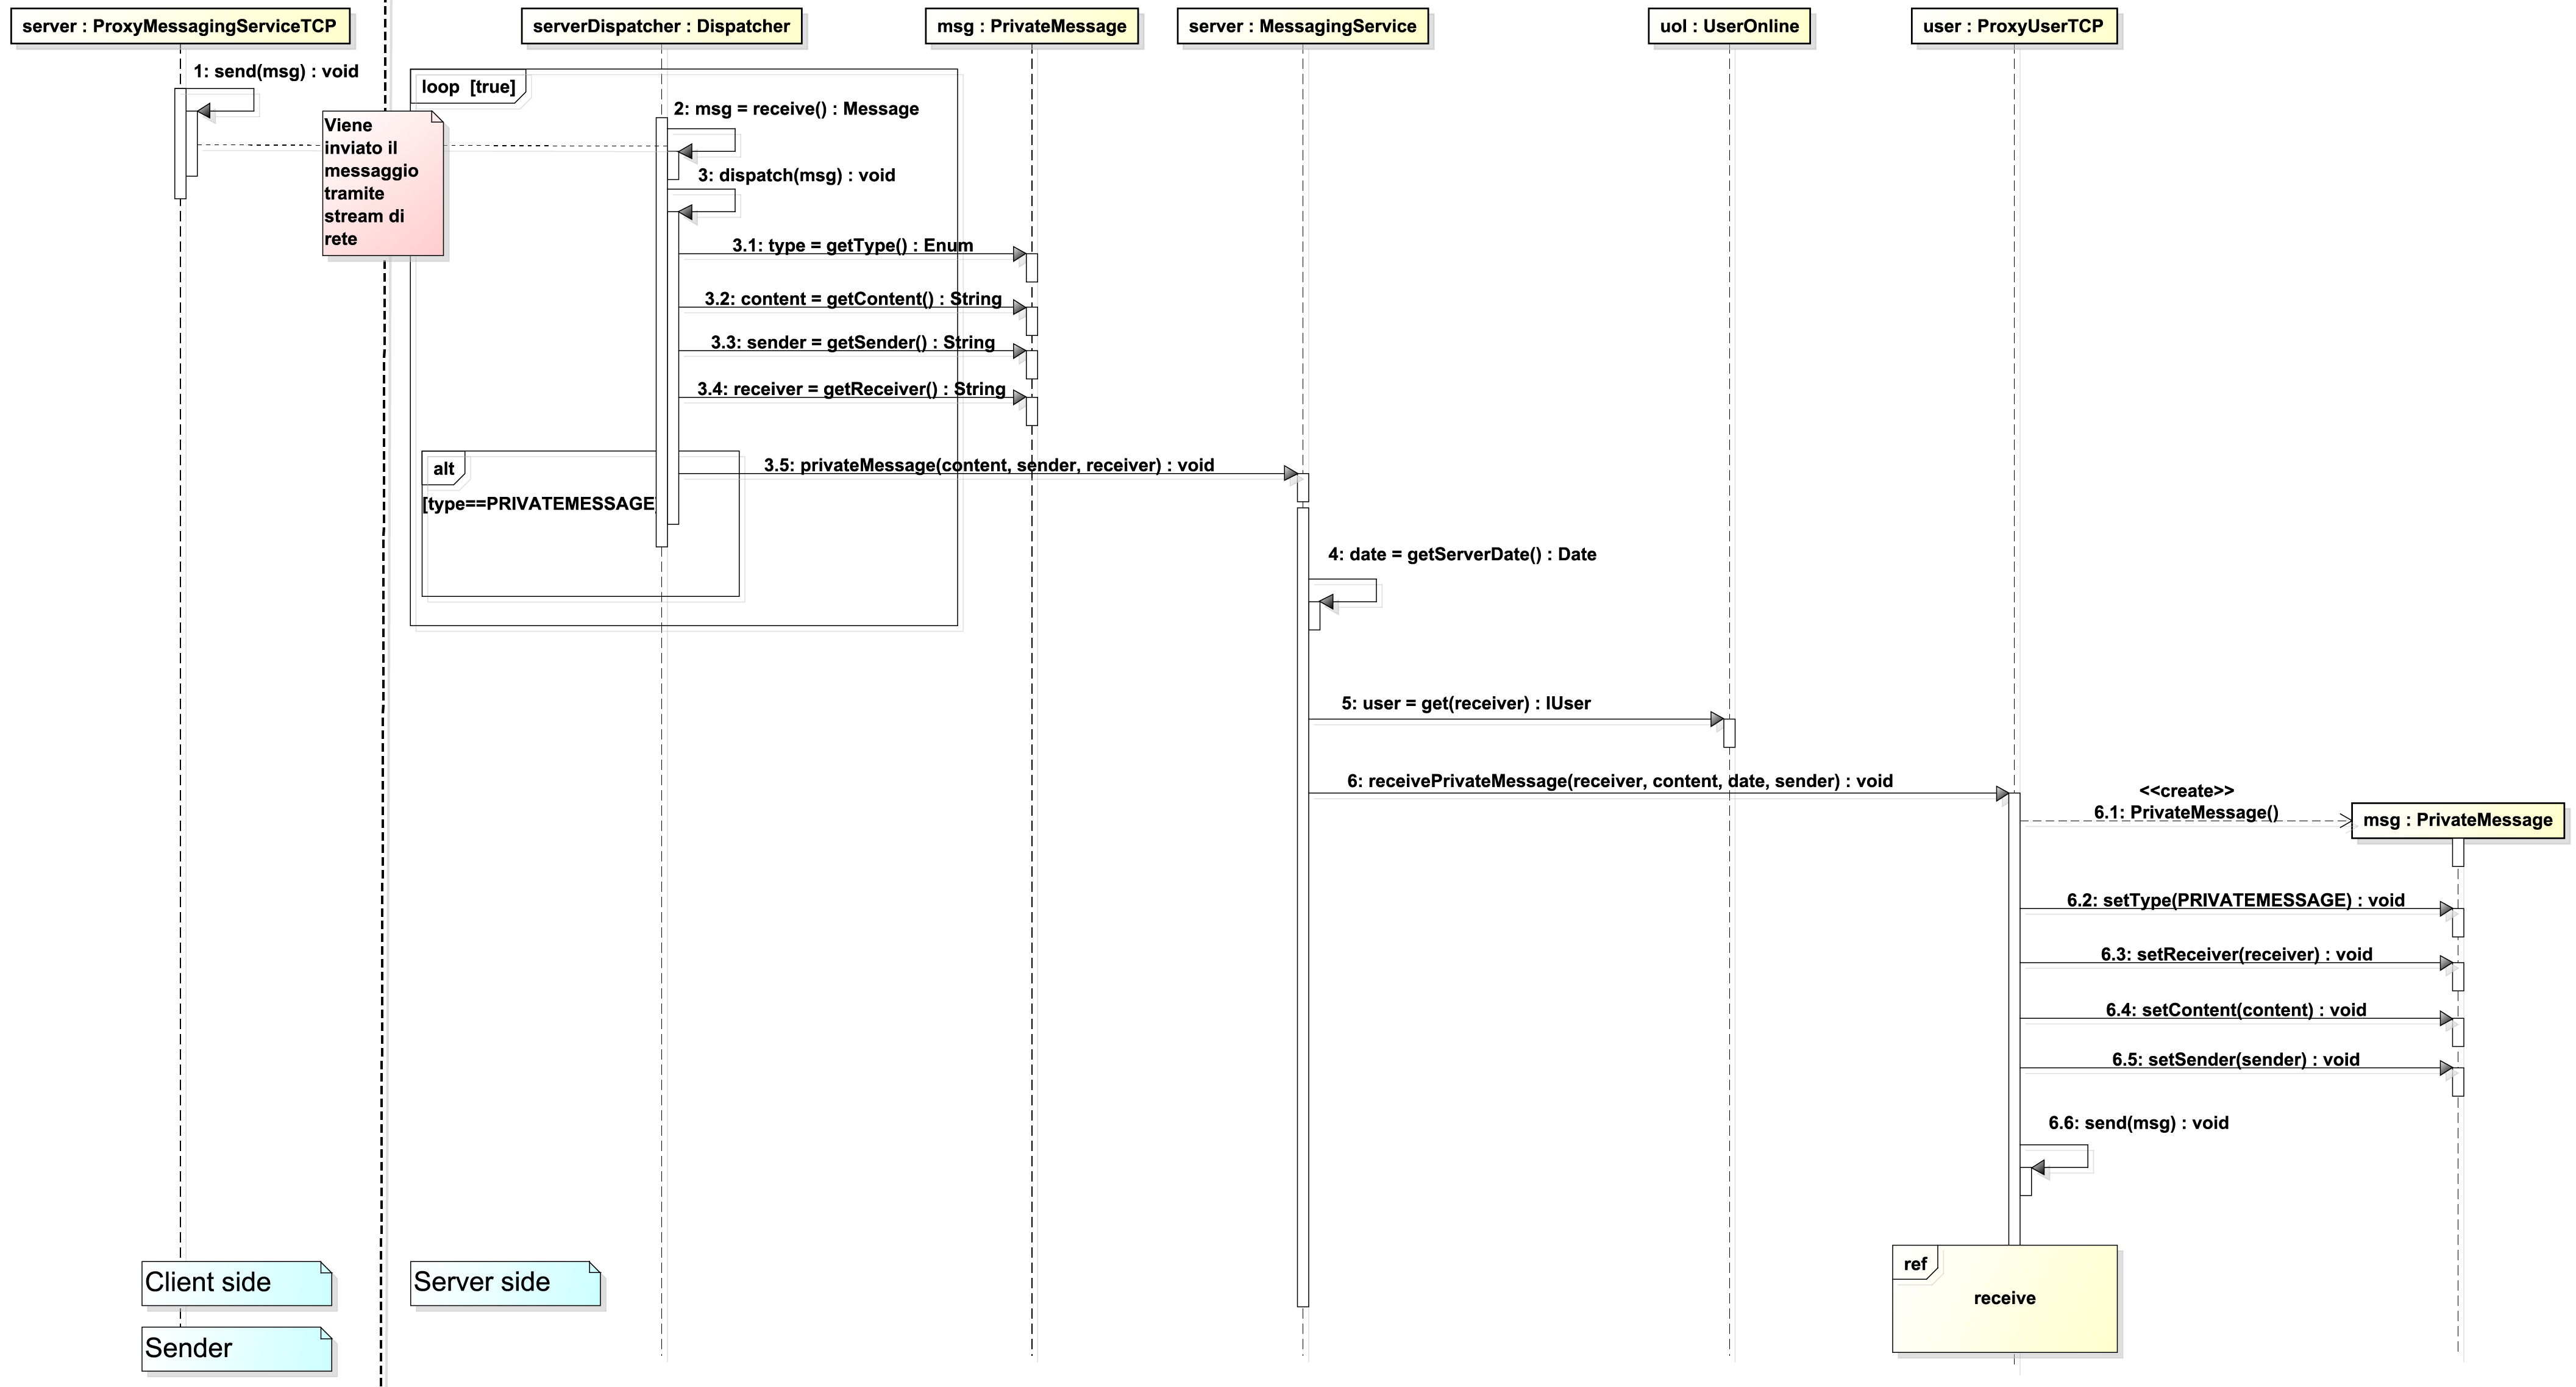
\includegraphics[scale=0.105]{image_astah/Iteration_3_DesignModel/UC4_SendPrivateMessage_SSD_2_privateMsg}{\centering}
     \caption{SSD - OP2: privateMsg(msg) del modello di dominio (figura \ref{fig_UC4_SPM_SSD}) }
     \label{fig_UC4_SSD_SRM_2} 
   \end{figure}
\end{frame}

\begin{frame} {Iterazione 3: Progettazione, UC4\_SendPrivateMessage - OP3}
   \begin{figure}
     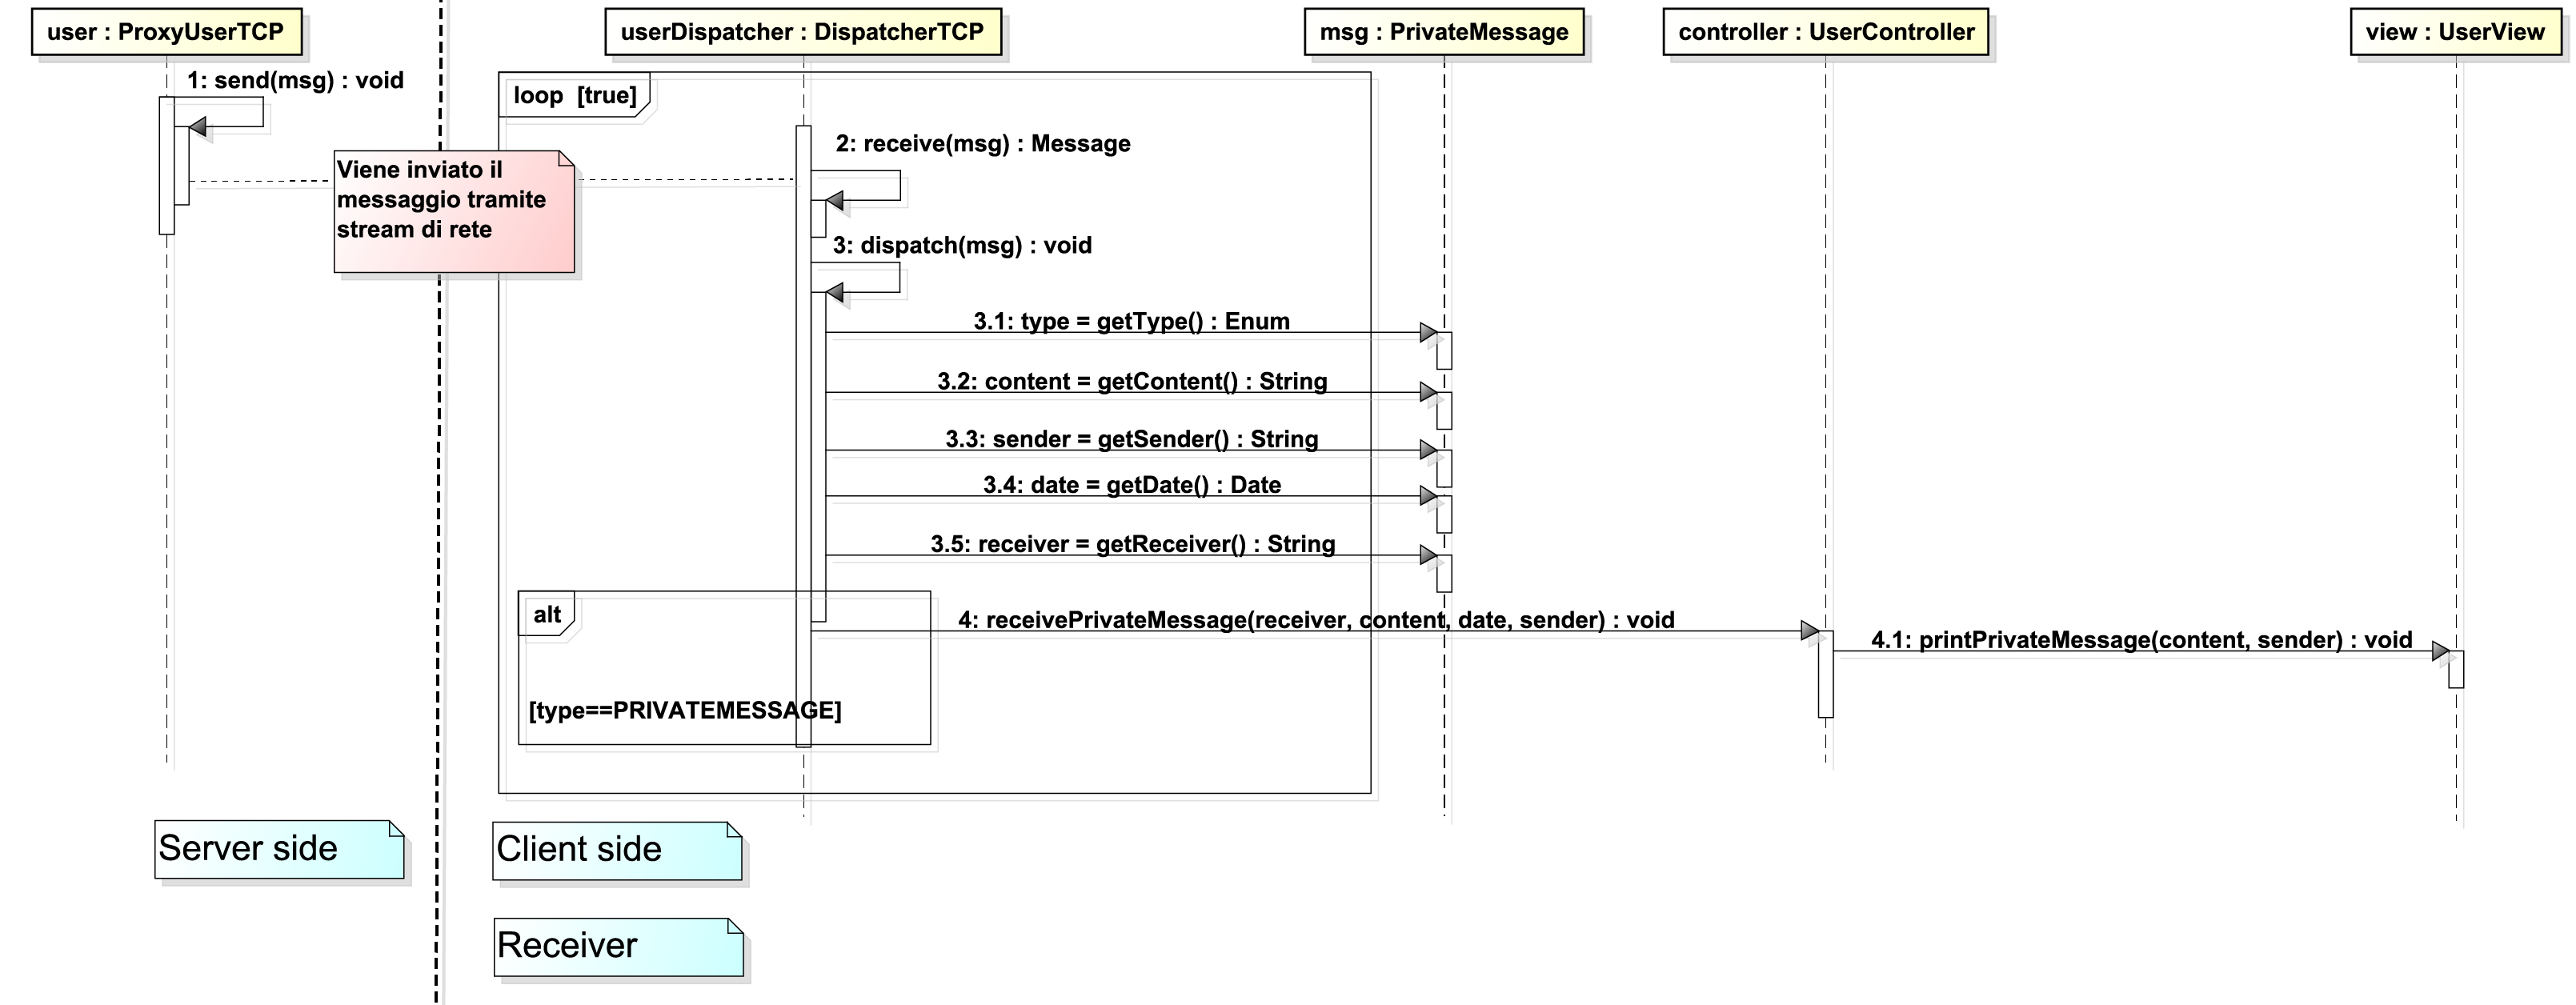
\includegraphics[scale=0.14]{image_astah/Iteration_3_DesignModel/UC4_SendPrivateMessage_SSD_3_receive.png}{\centering}
     \caption{SSD - OP3: receive(msg) del modello di dominio (figura \ref{fig_UC4_SPM_SSD})}
     \label{fig_UC4_SSD_SRM_3} 
   \end{figure}
\end{frame}


\subsection {Iterazione 3: Implementazione - UC4\_SendPrivateMessage}
\begin{frame} {Iterazione 3: Implementazione - UC4\_SendPrivateMessage}
 \emph{INSERIRE DESCRIZIONE}
\end{frame}

